\documentclass[nofootinbib,reprint,english]{revtex4-1}

% language
\usepackage[utf8]{inputenc}
\usepackage[english]{babel}

% standard setup
\usepackage{physics,amssymb,array}
\usepackage{xcolor,graphicx,hyperref}
\usepackage{tikz,listings,multirow}
\usepackage{algpseudocode,algorithm}
\usepackage{subcaption}
\usepackage{enumitem}

% tikz libraries
\usetikzlibrary{matrix}

% hyperref coloring
\hypersetup{ %
  colorlinks,
  linkcolor={red!50!black},
  citecolor={blue!50!black},
  urlcolor={blue!80!black}}

% lstlisting coloring
\lstset{ %
  inputpath=,
  backgroundcolor=\color{white!88!black},
  basicstyle={\ttfamily\scriptsize},
  commentstyle=\color{magenta},
  language=Python,
  tabsize=2,
  numbers=left,
  stringstyle=\color{green!55!black},
  frame=single,
  keywordstyle=\color{blue},
  showstringspaces=false,
  columns=fullflexible,
  keepspaces=true}

\DeclareTextSymbolDefault{\dh}{T1}

% no "do"'s or "then"'s
\algdef{SE}[FOR]{NoDoFor}{EndFor}[1]{\algorithmicfor\ #1}{\algorithmicend\ \algorithmicfor}
\algdef{SE}[FORALL]{NoDoForAll}{EndFor}[1]{\algorithmicfor\ #1}{\algorithmicend\ \algorithmicfor}
\algdef{SE}[IF]{NoThenIf}{EndIf}[1]{\algorithmicif\ #1}{\algorithmicend\ \algorithmicif}

% spin-configuration table columns
\newcolumntype{M}[1]{>{\centering\arraybackslash}m{#1}}
\newcolumntype{N}{@{}m{0pt}@{}}


\begin{document}
% titlepage
\title{FYS3150 Machine Learning - Project 3\\Classifying Pulsar Candidates With Machine Learning Methods}
\author{Nils Johannes Mikkelsen}
\date{\today}
\noaffiliation
\begin{abstract}
The project deals with the classification of pulsar candidates using statistical measures of the pulsar candidates' integrated pulse profile and the dispersion measure vs. signal-to-noise ratio curve. The classification is performed using both neural networks and support vector machines. Both methods are shown to produce excellent results with a highest accuracy score of 98\%, provided reasonable hyperparameters.
\end{abstract}
\maketitle
All material for project 3 may be found at:\\
{\scriptsize\url{https://github.com/njmikkelsen/machinelearning2018/tree/master/Project3}}\\
\section{Introduction}
In the field of radio astronomy, pulsars are among the most studied phenomena in nature. But despite astronomers' long history with puslars, little is actually known with certainty. However, much of the uncertainty likely boils down to the difficulty of confirming pulsar observations. While pulsars radiate unmistakable radio signals, they are often lost in the sheer number of radio signals observed by radio telescopes every day. Furthermore, due to the uniqueness of pulsar radio signals, classifying pulsars in large data sets of radio observations have historically been very difficult as human supervision has been a necessity. However, recent advancements in machine learning and data mining has made this task much simpler by introducing incredibly fast, in comparison to humans that is, classification methods. The aim of these machine learning methods is not to remove the role of the astronomer, but rather reduce large amounts of data to smaller, manageable data sets. If done effectively, such methods can be used a primary tool for extracting likely pulsar-candidates in order to survey large regions of the night sky in a fraction of the time.

\section{Theory}
\subsection{Radio Analysis of Pulsars}
The following theory is mostly based on F.G. Smith's 1977 \emph{Pulsars} \cite{Pulsars}, with additional information taken from ``Chapter 6: Pulsars'' of Jim Condon's online book \emph{Essential Radio Astronomy} \cite{EssentialRadioAstronomy}.

\subsubsection{The basics of pulsars}
Pulsars are heavily magnetised rotating astronomical objects that emit regular pulses of electromagnetic (EM) radiation. Initially discovered in 1967 by Antony Hewish and Jocelyn Bell Burnell, it is generally believed by most modern astronomers that pulsars are neutron stars, the product of some supernovae. There are several mechanims that result in the electromagnetic radiation (although still not entirely understood), astronomers have thus devised three major categories of pulsars according to the source of radiation: rotation-powered pulsars, accretion-powered pulsars and magnetars. Rotation-powered pulsars use the loss of rotational energy, accretion-powered pulsars exploit the gravitational potential energy of accreted matter, while magnetars are believed to power its radiation pulses by the decay of an extremely strong magnetic field (\(\sim10^{10}\) T). Other than regular pulses of radiation, the properties of the radiation from the different categories are mostly different. Rotation-powered pulsars radiate mostly in the Radio spectrum, while the accretion-powered pulsars radiate mostly in the X-Ray spectrum. Magnetars have been observed to radiate both in the X-Ray and gamma-ray spectra.

The data studied in this project stem from radio-telescope observations, thus only rotation-powered pulsars are considered here.
\subsubsection{ISM dispersion}
As the name implies, radio pulsars are particular pulsars that radiate in the radio spectrum. When astronomers first began studying radio pulsars they noticed that radiation from the same pulsar with different frequencies arrived on Earth at different times. It was quickly pointed out that this EM dispersion coincided with the expected dispersion of EM waves travelling through the cold plasma of the interstellar medium (ISM). Travelling through an ionised gas, the group and phase velocities of radio waves, \(v_g\) and \(v_p\) respectively, are related by
\begin{equation}\label{eq:group_and_phase_velocities_cold_plasma}
v_gv_p=c^2
\end{equation}
where \(c\) is the speed of light in a vacuum. The fractive index of the cold plasma is
\begin{equation}\label{eq:refractive_index_cold_plasma}
\mu=\sqrt{1-\Big(\frac{\nu_\text{p}}{\nu}\Big)^2}
\end{equation}
where \(\nu\) is the radio wave frequency and \(\nu_\text{p}\) is the \emph{plasma frequency} given by:
\begin{equation}
\nu_\text{p}=\sqrt{\frac{e^2n_e}{\pi m_e}}
\end{equation}
Here, \(n_e\) and \(m_e\) are the electron number density and \(m_e\) is the electron mass. Now, radio waves with \(\nu\leq\nu_\text{p}\) are unable to propegate through the ISM. On the other hand, waves with \(\nu>\nu_\text{p}\) do propegate through the ISM with a group velocity of
\begin{equation}\label{eq:radio_wave_group_velocity_propegation}
v_g=\mu c\cong\bigg(1-\frac{\nu_\text{p}^2}{2\nu^2}\,\bigg)c
\end{equation}
Hence, the travel time \(T\) spent by a radio pulse from a pulsar a distance \(L\) away is
\begin{align}
T&=\int_0^L\frac{1}{v_g}\dd{l}=\frac{1}{c}\int_0^L\bigg(1+\frac{\nu_\text{p}^2}{2\nu}\bigg)\dd{l}\nonumber\\
&=\frac{d}{c}+\bigg(\frac{e^2}{2\pi m_ec}\bigg)\nu^{-2}\int_0^L n_e\dd{l}\label{eq:radio_wave_travel_time}
\end{align}
The integral in \eqref{eq:radio_wave_travel_time} is commonly called the \emph{Dispersion Measure}, and is commonly given in units of pc \(\text{cm}^{-3}\):
\begin{equation}\label{eq:Dispersion_Measure}
\text{DM}=\int_0^Ln_e\dd{l}
\end{equation}
The Dispersion Measure is not a trivial quantity to estimate because it depends on the constituents and their arrangements of the ISM, which in general is not uniform. Despite accurate theoretical predictions of DM, it continues to be an essential variable parameter in radio astronomy analysis, more or this below. In astronomy-convenient units, the dispersion delay \(t=T-d/c\) due to the ISM is
\begin{equation}\label{eq:ISM_dispersion_delay}
t\cong4.149\cdot10^3\nu^{-2}\,\text{DM}\text{ seconds}
\end{equation}
where \(\nu\) in MHz and DM in pc \(\text{cm}^{-3}\).
\subsubsection{The integrated pulse profile}
Due to difficulties with time-resolution, limited bandwidth, etc., studying a single radio pulse is considerably more difficult than to study the ``average pulse'' across several frequencies. Taking into account the time delay due to dispersion in the ISM (equation \eqref{eq:ISM_dispersion_delay}), the radio pulses from radio pulsars may be \emph{folded} to yield an ``\emph{integrated pulse profile}'' (IPP). Seeing that the DM is essential in the computation of the time delay, astronomers often study the IPP as a function of DM. An example of the folding process is shown in figure \ref{fig:integrated_pulse_profile}, note that the delay folds across several pulse periods. Moreover, while the time-signal is fairly chaotic, the integrated pulse profile is very focused.

While all pulsars share the property of a stable pulse profile, it turns out that each pulsar exhibits a particular profile that is more or less unique. This unique profile, often nicknamed the ``fingerprint'' of the pulsar, can have several peaks and be less or more spread out. Nonetheless, some statistical properties such as a single peak, a double peak, various minor peaks, etc., do occur quite frequently.

\begin{figure}
\centering
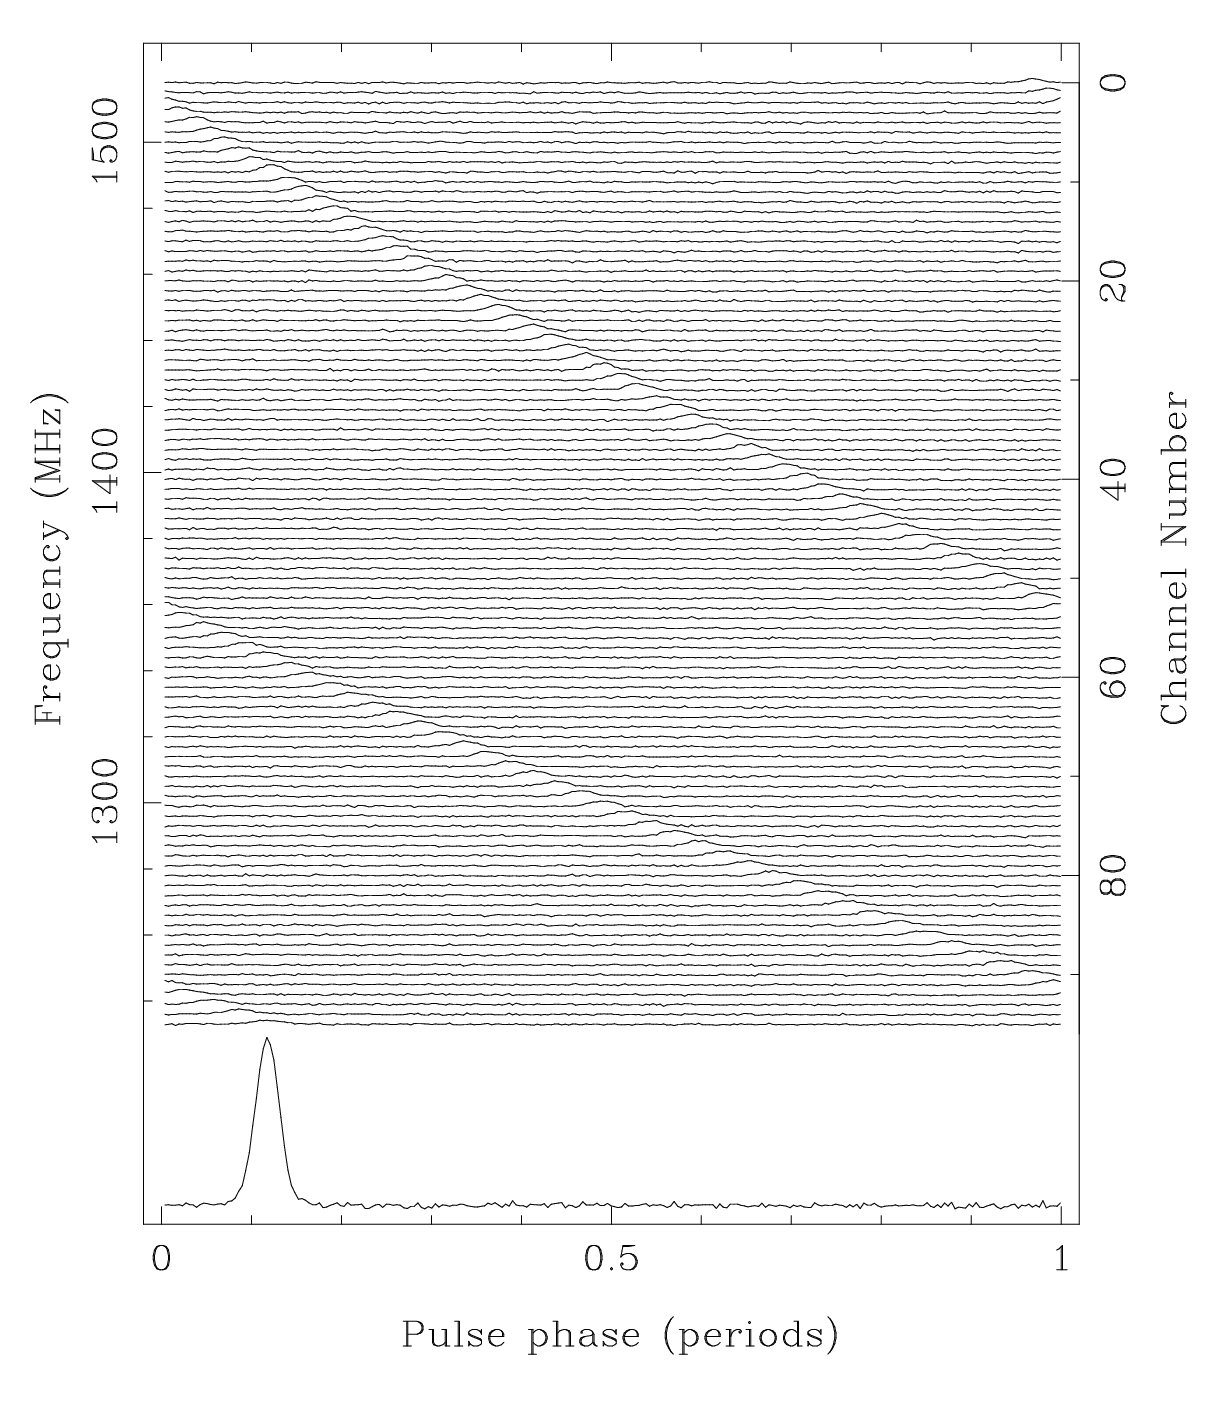
\includegraphics[scale=0.2]{./Pulsar_dm.png}
\caption{The pulse profile of a radio wave experiences a time delay due to dispersion in the ISM. The integrated pulse profile is a folded profile that finds an average pulse profile by taking into account the time delay. Source: \cite{IntegratedPulseProfile}}\label{fig:integrated_pulse_profile}
\end{figure}

\subsubsection{Signal-to-noise ratio}
An important quantity in observational astronomy is the Signal-to-Noise Ratio (SNR), which in its simplest form is defined as the ratio of the power of the signal to the power of the noise:
\begin{equation}
\text{SNR}=\frac{P_\text{signal}}{P_\text{noise}}
\end{equation}
SNR is a measure of the quality of observation, or ``amount of meaningful information'' in an observation. Astronomers actually use the SNR to study the DM parameter space, as selecting the optimal DM is essential for conducting a proper analysis of the IPP. Enter the the DM-SNR curve: the SNR score of an integrated pulse profile as a function of DM. The DM-SNR curve is usually flat for non-pulsating signals, however peaks about the optimal DM if the signal does pulsate. Consequently, the DM-SNR curve is commonly used as a preliminary test for identifying signals from pulsars in large data sets of radio signals.

\subsection{Moments In Statistics}
Given some continuous function \(f:\mathbb{R}\to\mathbb{R}\), its \(n^\text{th}\) \emph{moment} \(\mu_n(c)\) about the real value \(c\) is defined as
\begin{equation}\label{eq:moments}
\mu_n(c)=\int_{-\infty}^\infty(x-c)^nf(x)\dd{x}
\end{equation}
Moments are used in several areas of science and mathematics, most prominently in mechanics and probability theory. If \(f\) is a probability density (or strictly non-negative and normalizable),\footnote{A probability density \(f:D\to\mathbb{R}\) satifies
\[0\leq f(x),\ \forall x\in D\qand\int_Df(x)\dd{x}=1.\]
Note that \(D\) is usually the entire real number line.} there exists two major notation conventions:
\[\mu_n(c)=E\big[(X-c)^n\big]\qand\mu_n(c)=\expval{(x-c)^n}\]
The former is favoured by statisticians, while the latter is favoured by physicists, this project will employ the physicists' convention.

The moments most often studied in probability theory are the so-called \emph{central} moments \(\mu_n\):
\begin{equation}\label{eq:central_moments}
\mu_n=\mu_n(\mu)=\expval{(x-\mu)^n}=\int_{-\infty}^\infty(x-\mu)^nf(x)\dd{x}
\end{equation}
where \(\mu=\expval{x}\) is the mean value of the distribution and \(\mu_n=\mu_n(\mu)\) is introduced to simplify notation. The \(0^\text{th}\) and \(1^\text{st}\) central moments are 1 and 0 respectively as \(f(x)\) is normalized and \((x-\mu)f(x)\) is centered about \(\mu\). The \(2^\text{nd}\) central moment is the variance:
\begin{equation}
\mu_2=\expval{(x-\mu)^2}=\sigma^2
\end{equation}
where \(\sigma\) is the standard deviation.

Furthermore, the central moments are used to define the \emph{normalized} moments \(\tilde{\mu}_n\):
\begin{equation}
\tilde{\mu}_n=\frac{\mu_n}{\sigma^n}=\frac{\expval{(x-\mu)^n}}{\expval{(x-\mu)^2}^{n/2}}
\end{equation}
Normalized moments are dimensionless quantities that describe the underlying distribution independently of the scale of the data. The \(3^\text{rd}\) normalized moment is known as the \emph{skewness} of a distribution and quantifies the extent to which a distribution is \emph{skewed} to ``left or right'' of the mean. Positive skewness implies the distribution is skewed towards \(x\) values greater than \(\mu\) and vice versa. The \(4^\text{th}\) normalized moment is called \emph{kurtosis} and is a measure of how quickly the tails of a distribution tends to zero, i.e. a measure of ``\emph{peakness}''. Kurtosis is usually reported as \emph{excess kurtosis}, which is the kurtosis of a distribution relative to the normal distribution (whose kurotsis is 3). Hence the definition:
\begin{equation}
\text{Excess Kurtosis }=\text{ Kurtosis}-3
\end{equation}
\subsection{Machine Learning - Artificial Neural Networks}
Artificial Nerual Networks (ANN or simply NN) is a Supervised Machine Learning (SML) technique that is inspired by biological neural networks in animal brains. Rather than a specific technique or algorithm, ANN is an umbrella term for several NN structures and algorithms whose complexity, computational difficulty, etc., varies greatly between different techniques.
\subsubsection{The Multi-Layered Perceptron}
This project will employ the so-called Multi-Layered Perceptron (MLP) model, which is a particular ANN that is based around the idea of organizing the network's neurons, or nodes, in layers. A node is loosely based on the concept of biological neuron, which is capable of recieving an electrical signal, process it, and transmit a new signal to other neurons. In the MLP model the neurons are arranged in \(L\) consecutive layers with \(N_l\) number of nodes per layer (unqeual number of nodes per layer is alloweed).  There are three types of layers: input, hidden and output layers. The input and output layers manage the network's inputs and outputs, while the hidden layers serve as the network's data-processing backbone. Particular to the MLP, every node in each hidden layer is connected to every node in the previous and the next layers, but nodes within the same layer are \emph{not} connected. The MLP structure is illustrated in figure \ref{fig:node_connections}, note the inclusion of ``bias'': Bias is an additional property of all layers except the input layer whose purpose is essentially to center the data about 0. Conceptually, one may think of bias as the role of the intercept in Linear Regression analysis.

\begin{figure}
\centering
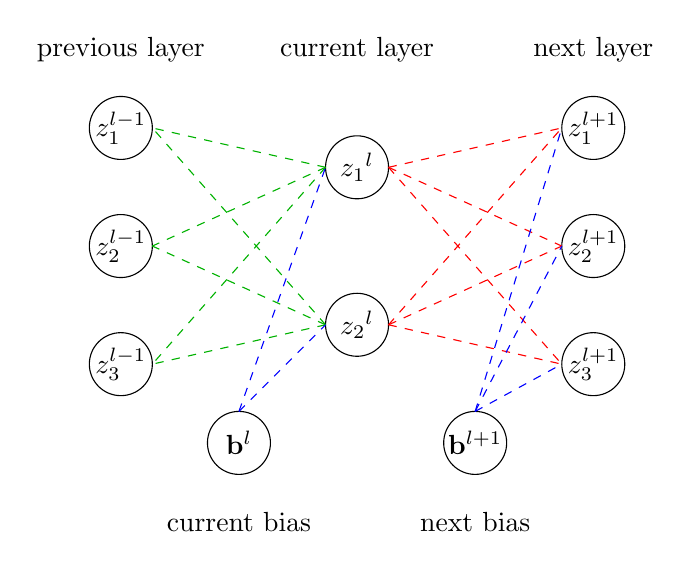
\begin{tikzpicture}
% NODES
\draw node at (-3,2.5) {previous layer};
\draw (-3,+1.5) circle [radius=0.4];
\draw (-3,+0.0) circle [radius=0.4];
\draw (-3,-1.5) circle [radius=0.4];

\draw node at (-1.5,-3.5) {current bias};
\draw (-1.5,-2.5) circle [radius=0.4];

\draw node at (+0,2.5) {current layer};
\draw (+0,+1.0) circle [radius=0.4];
\draw (+0,-1.0) circle [radius=0.4];

\draw node at (+1.5,-3.5) {next bias};
\draw (+1.5,-2.5) circle [radius=0.4];

\draw node at (+3,2.5) {next layer};
\draw (+3,+1.5) circle [radius=0.4];
\draw (+3,+0.0) circle [radius=0.4];
\draw (+3,-1.5) circle [radius=0.4];
% CONNECTIONS
\draw[dashed,red] (+0.4,+1.0) -- (+3-0.4,+1.5);
\draw[dashed,red] (+0.4,+1.0) -- (+3-0.4,+0.0);
\draw[dashed,red] (+0.4,+1.0) -- (+3-0.4,-1.5);

\draw[dashed,red] (+0.4,-1.0) -- (+3-0.4,+1.5);
\draw[dashed,red] (+0.4,-1.0) -- (+3-0.4,+0.0);
\draw[dashed,red] (+0.4,-1.0) -- (+3-0.4,-1.5);

\draw[dashed,green!70!black] (-0.4,+1.0) -- (-3+0.4,+1.5);
\draw[dashed,green!70!black] (-0.4,+1.0) -- (-3+0.4,+0.0);
\draw[dashed,green!70!black] (-0.4,+1.0) -- (-3+0.4,-1.5);

\draw[dashed,green!70!black] (-0.4,-1.0) -- (-3+0.4,+1.5);
\draw[dashed,green!70!black] (-0.4,-1.0) -- (-3+0.4,+0.0);
\draw[dashed,green!70!black] (-0.4,-1.0) -- (-3+0.4,-1.5);

\draw[dashed,blue] (+1.5,-2.5+0.4) -- (+3.0-0.4,+1.5);
\draw[dashed,blue] (+1.5,-2.5+0.4) -- (+3.0-0.4,+0.0);
\draw[dashed,blue] (+1.5,-2.5+0.4) -- (+3.0-0.4,-1.5);

\draw[dashed,blue] (-1.5,-2.5+0.4) -- (-0.4,+1.0);
\draw[dashed,blue] (-1.5,-2.5+0.4) -- (-0.4,-1.0);
% NODE NAMES
\draw node at (+0.0,+1.0) {\({z_1}^l\)};
\draw node at (+0.0,-1.0) {\({z_2}^l\)};

\draw node at (+3.0,+1.5) {\(z_1^{l+1}\)};
\draw node at (+3.0,+0.0) {\(z_2^{l+1}\)};
\draw node at (+3.0,-1.5) {\(z_3^{l+1}\)};

\draw node at (-3.0,+1.5) {\(z_1^{l-1}\)};
\draw node at (-3.0,+0.0) {\(z_2^{l-1}\)};
\draw node at (-3.0,-1.5) {\(z_3^{l-1}\)};

\draw node at (+1.5,-2.5) {\(\vb{b}^{l+1}\)};
\draw node at (-1.5,-2.5) {\(\vb{b}^l\)};
\end{tikzpicture}
\caption{An illustration of the structure of an MLP ANN: Each node is connected to every node in the previous layer and the next layer. The inputs to the current layer consists of the data from the previous layer (green connections) and the current layer's bias (left blue connections). The outputs of the current layer (red connections) together with the next layer's bias (right blue connections) become the inputs of the next layer, and so on.}\label{fig:node_connections}
\end{figure}

So far the network has only been described using fluid terms such as ``transfer of information'' and ``node connections'', this will be expanded upon now. The number of nodes in the input layer \(N_1\) must exactly match the dimensionality of the input data, thus there is a one-to-one correspondence between the nodes and the indices of the input data (usually a vector quantity). Similarly, the number of nodes in output layer \(N_L\) must exactly match the output data of the network, again with a one-to-one correspondence between nodes and data indices. It follows that in practice it is really only the hidden layers that may have a variable number of nodes \(N_l\), \(l\in\{2,\ldots,L-1\}\). The network processes input data layer-by-layer, meaning each hidden layer processes the data in sequence. Data from the input layer is sent to the first hidden layer, processed, then transfered to the next layer, and so on.

Mathematically speaking, the connection between two nodes \(i\) in layer \(l\) and \(j\) in layer \(l+1\) is a scaling operation. The connection's scaling factor is usually called the weight and is commonly denoted by \(w_{ij}^{l+1}\), note the convention of labeling a connection weight between layers \(l\) and \(l+1\) by \(l+1\). Each node is connected to every node in the previous layer, thus the purpose of weighting the data is to regulate the importance of each node in the previous layer. However, note that unless some other operation is conducted on the data the network's overall operation on the input data is only linear (meaning methods such as Linear Regression are more appropriate). This is circumvented by the addition of a non-linear operation on the every node's input, commonly called the node's \emph{activation} function. Common activation functions include:
\begin{subequations}
\begin{align}
\text{logistic}(x)&=\frac{1}{1+e^{-x}}\\
\text{sigmoid}(x)&=\tanh(x)\\
\text{rectifier}(x)&=\max(0,x)
\end{align}
\end{subequations}
Other activation functions are also used. Technically, a network may have a different activation for each node, but this is rarely done in practice. On the other hand, layer-wide activation functions are often implemented, so much so that the following theory will base the mathematics on the presumption of layer-wide activation.

The data in node \(i\) in layer \(l\) is denoted by \(y_i^l\). The connection weight between node \(i\) in layer \(l\) and node \(j\) in layer \(l+1\) is denoted by \(w_{ij}^{l+1}\). The accumulated data input from all nodes in layer \(l\) received by node \(j\) in layer \(l+1\), adjusted for bias \(b_j\), is given by
\begin{equation}\label{eq:neural_network_node_received_data}
z_j^{l+1}=\sum_{i=1}^{N_l}w_{ij}^{l+1}y_i^l+b_i^l
\end{equation}
The input data received by the node is \(f_{l+1}(z_j^{l+1})\), where \(f_{l+1}\) is the activation function of layer \(l+1\). Hence, the data in node \(j\) in layer \(l+1\) is given by
\begin{equation}\label{eq:neural_network_node_data}
y_j^{l+1}=f_{l+1}(z_j^{l+1})=f_{l+1}\Bigg(\sum_{i=1}^{N_l}w_{ij}^{l+1}y_i^l+b_j^{l+1}\Bigg)
\end{equation}
Arranging the node data in vectors \(\vb{y}^l\), the node inputs in vectors \(\vb{z}^{l+1}\), the connection weights in a weight matrix \(\hat{W}^{l+1}\) and the bias in bias vectors \(\vb{b}^{l+1}\), then \eqref{eq:neural_network_node_data} can be reformulated as a layer-wide (matrix) operation:
\begin{equation}\label{eq:neural_network_layer_input}
\vb{y}^{l+1}=f_{l+1}(\vb{z}^{l+1})=f_{l+1}\Big(\hat{W}^{l+1}\vb{z}^l+\vb{b}^{l+1}\Big)
\end{equation}
To conclude this section: The answer to the question \emph{"What is a Multi-Layered Perceptron Neural Network?"} is the following function:
\begin{equation}\label{eq:equation_of_neural_network}
\vb{y}=f_L\bigg(\hat{W}^Lf_{L-1}\bigg(\cdots \bigg(\hat{W}^1\vb{x}+\vb{b}^1\bigg)\cdots\bigg)+\vb{b}^L\bigg)
\end{equation}
where \(\vb{x}=\vb{y}^1\) and \(\vb{y}=\vb{y}^L\) are the network's inputs and outputs.
\subsubsection{Training an MLP}
The basis of the MLP, and many similar network structures, is the so-called \emph{back-propagation} algorithm (BPA). The MLP is an example of a \emph{supervised} machine learning technique, meaning the desired outputs are known. In case of the MLP, it is the BPA that introduces supervision.

At its core, the BPA is essentially a variant of gradient descent techniques. The basic problem of gradient descent methods is to find the input \(\vb{x}_\text{min}\in D\) that minimises some function \(F:D\to\mathbb{R}\). The algorithm is based on producing sucessive approximations of \(\vb{x}_\text{min}\), each closer to the true minium. Seeing that the goal is to minimise \(F\), the direction of each step is chosen opposite of the gradient of \(F\). The fundamental algorithm is summarised below:
\begin{algorithm}[H]
\caption{Gradient Descent}\label{alg:gradient_descent}
\begin{algorithmic}[1]
\State Select a trial input \(\vb{x}_0\).
\NoDoFor {\(i=1,\ldots,N\):}
	\State Compute: \(\displaystyle\vb{x}_i=\vb{x}_{i-1}-\gamma_i\pdv{F}{\vb{x}}\eval_{\vb{x}_{i-1}}\)
\EndFor
\end{algorithmic}
\end{algorithm}
\noindent Note that the derivative is not scalar. The step length \(\gamma_n\) may be variable or constant depending on the implementation, although proper convergence is impossible with too large steps.

The \(F\) function to minimise in the BPA is the so-called \emph{cost} function, denoted \(C\). Similar to activation functions, different cost functions are used in different problems. The cost function most used in classification analysis is the so-called cross-entropy:
\begin{equation}\label{eq:cross_entropy_MLP}
C(\vb{y}|\vb{t})=-\Big[\vb{t}^T\ln(\vb{y})+(1-\vb{t})^T\ln(1-\vb{y})\Big]
\end{equation}
where \(\vb{y}\) is a vector of the network's outputs and \(\vb{t}\) is a vector of the targets, i.e. the desired network output.\footnote{The introduction of \(\vb{t}\) in the cost function is the actual introduction of machine learning supervision in MLP ANNs. Also, note that naming \(\vb{t}\) the ``targets'' refers to the goal of neural networks: namely to construct the network such that it reproduces the target outputs.} Note that \(C(\vb{y}|\vb{t})\) is univariate: it is a function of outputs \(\vb{y}\) provided the targets \(\vb{t}\) (that is, \(\vb{t}\) is not a variable quantity). The derivative of \(C(\vb{y}|\vb{t})\) is
\begin{equation}\label{eq:cross_entropy_derivative_MLP}
\pdv{C}{\vb{y}}=(\vb{y}-\vb{t})\oslash\Big(\vb{y}\circ(1-\vb{y})\Big)
\end{equation}
where \(\oslash\) and \(\circ\) denotes the Hadamard division and product (element-wise operations). Now, if this was a problem for gradient descent methods, then \(\vb{y}\) would be updated directly using Algorithm \ref{alg:gradient_descent} and equation \eqref{eq:cross_entropy_derivative_MLP}. However, \(\vb{y}\) is produced by the network according to equation \eqref{eq:equation_of_neural_network}, which is dependent on the weights and biases of each layer. Hence, in order for the BPA to improve the network it must study \(C(\vb{y}|\vb{t})\) with respect to all weights and biases. 

Although seemingly difficult, the problem is actually somewhat straight-forward, it all comes down to clever use of the chain rule and limiting the number of necessary computations. Observe that the derivative of \(C(\vb{y}|\vb{t})\) with respect to layer \(l\) can be written as
\begin{subequations}\label{eq:cost_derivative_layer_l_standard}
\begin{align}
\pdv{C}{\hat{W}^l}&=\pdv{C}{\vb{y}^l}\,\pdv{\vb{y}^l}{\vb{z}^l}\,\pdv{\vb{z}^l}{\hat{W}^l}\\
\pdv{C}{\vb{b}^l}&=\pdv{C}{\vb{y}^l}\,\pdv{\vb{y}^l}{\vb{z}^l}\,\pdv{\vb{z}^l}{\vb{b}^l}
\end{align}
\end{subequations}
Now define the \emph{signal error} of layer \(l\) as
\begin{equation}\label{eq:signal_error_definition}
\hat{\delta}^l\equiv\pdv{C}{\vb{z}^l}=\pdv{C}{\vb{y}^l}\,\pdv{\vb{y}^l}{\vb{z}^l}=\pdv{C}{\vb{y}^l}\circ f'_l(\vb{z}^l)
\end{equation}
where \(f'_l(\vb{z}^l)\) is the derivative of the activation function of layer \(l\). Clearly then equations \eqref{eq:cost_derivative_layer_l_standard} may be written as
\begin{subequations}\label{eq:cost_derivative_layer_l}
\begin{align}
\pdv{C}{\hat{W}^l}&=\hat{\delta}^l\vb{y}^{l-1}\\
\pdv{C}{\vb{b}^l}&=\hat{\delta}^l
\end{align}
\end{subequations}
where \(\vb{z}^l=\hat{W}^l\vb{y}^{l-1}+\vb{b}^l\) was used to evalute \(\partial\vb{z}^l/\partial\hat{W}^l\) and \(\partial\vb{z}^l/\partial\vb{b}^l\). The next step is to relate the signal error of layer \(l\) to \(l+1\), the idea to rewrite \(\partial C/\partial\vb{y}^l\) in \eqref{eq:signal_error_definition} using a reverse chain rule:\footnote{The awkward double-transpose notation is used to preserve the correct dimensions of \(\partial C/\partial\vb{y}^l\).}
\[\pdv{C}{\vb{y}^l}=\pdv{C}{\vb{z}^{l+1}}\,\pdv{\vb{z}^{l+1}}{\vb{y}^l}=\Big[\big(\hat{\delta}^{l+1}\big)^T\hat{W}^{l+1}\Big]^T=\big(\hat{W}^{l+1}\big)^T\hat{\delta}^{l+1}\]
That is, the signal error of layer \(l\) is related to the signal error of layer \(l+1\) via
\begin{equation}\label{eq:signal_error_recursive_relation}
\hat{\delta}^l=\big(\hat{W}^{l+1}\big)^T\hat{\delta}^{l+1}\circ f'_l(\vb{z}^l)
\end{equation}

Equations \eqref{eq:cost_derivative_layer_l}, \eqref{eq:signal_error_definition} and \eqref{eq:signal_error_recursive_relation} are what constitutes the \emph{four equations of the back-propagation algorithm}. The equations essentially boil down to the equivalent of step 3 in Algorithm \ref{alg:gradient_descent} (in particular \eqref{eq:cost_derivative_layer_l}). Moreover, note that the ``back-propagated quantity'' in the BPA is the signal error, i.e., the network's output error is propagated backwards through the network (thereby expressing the dependency of the cost function on the signal error of the different layers).

The back-propagation algorithm is composed of 3 steps: the feed forward cycle, the back-propagation and the network update. The feed forward step refers to the computation of the network's output; the input data \(\vb{x}\) is ``fed forward'' to the output. The back-propagation step involves the computation of the signal errors and the final network update is the updating of the network's weights and biases using the derivatives of the cost function. The full algorithm is shown below. 

\begin{algorithm}[H]
\caption{The Back-Propagation Algorithm}\label{alg:back_propagation}
\begin{algorithmic}[1]
\State Initiate the network weights and biases.
\NoDoFor {\(i=1,\ldots,N\):}
	\State Feed forward input \(\vb{x}\).
	\State Compute \(\hat{\delta}^L\).
	\NoDoFor {\(l=L-1,\ldots,1\):}
		\State Compute \(\hat{\delta}^l\).
	\EndFor
	\State Update the network weights and biases according to
\begin{align*}
\hat{W}^l_\text{next}&=\hat{W}^l_\text{prev}-\gamma_i\pdv{C}{\hat{W}^l_\text{prev}}\\
\vb{b}^l_\text{next}&=\vb{b}^l_\text{prev}-\gamma_i\pdv{C}{\vb{b}^l_\text{prev}}
\end{align*}
\EndFor
\end{algorithmic}
\end{algorithm}

\subsubsection{MLP Classifiers}
The MLP network described up until now technically does not perform a classification, but a regression. This is not a problem however as adjusting the network to function as a classifier is not particularly difficult. The only meaningful difference is in the output layer, in particular the output layer activation function.

The most common choice of ouput layer activation for classification problems is the softmax function:
\begin{equation}
\text{softmax}(\vb{x},i)=\frac{e^{x_i}}{\sum_{j=1}^Ne^{x_j}}
\end{equation}
where \(\vb{x}\) is a vector of \(N\) components. The reason why the softmax is so popular is that it is normalized: \(\sum_i^N\text{softmax}(\vb{x},i)=1\), which is an important property with regards to probability. The idea to use the MLP network as a regression model to produce probabilities, and in turn classify the input data according to the most likely classes.

\subsubsection{Improving BPA convergence}
First and foremost, it is very difficult to predict how the BPA behaves with respect to a contant learning rate. Hence, a guarantee of convergence is much more likely if the learning rate is adjusted during the iteration. For the time being, no particular updating scheme seems to be universally optimal. The updating scheme used in this project is the so-called ``\emph{adaptive scheme}'', which updates the learning rate if the cost function is not improved after \(n\) iterations. This project will update the learning rate if 10 consecutive iterations fail to improve the cost via:
\begin{equation}
\gamma_{n+1}=\frac{\gamma_n}{5}
\end{equation}

As it stands, notice that Algorithm \ref{alg:back_propagation} makes no mention of the possibility of multiple data inputs \(x\). A simple way to accomodate several data samples would be to iterate over the available samples \(\vb{x}_i\) within the BPA loop. However, this is very error-prone as it is likely to favour the first samples (especially with the adaptive learning rate). This can be slightly improved by using a stochastic approach, meaning the samples are picked at random. Nevertheless, this would only choose ``the first samples'' stochastically, not fix the underlying problem. A better approach is to use the average of several samples chosen at random, which means the mathematics must be somewhat adjusted (although not much): The input vector \(\vb{x}\) is replaced by an input matrix \(\vb{X}=\mqty[\vb{x}_1&\cdots&\vb{x}_M]\), which implies that the vector quantities \(\hat{\delta}^l\), \(\vb{z}^l\) and \(\vb{y}^l\) now become equivalent matrix quantities. Both \(\hat{W}^l\) and \(\vb{b}^l\) remain the same. Finally \(\hat{\delta}^l\) is reduced from a matrix of column vectors to the average column vector before being used to compute \(\partial C/\partial\hat{W}^l_\text{prev}\) and \(\partial C/\partial\vb{b}^l_\text{prev}\). What remains now is to select the set of input vectors to use in \(\vb{X}\). Including all vectors usually leads to too large matrices, and is also sensitive to outliers. The so-called \emph{Stochastic Gradient Descent} (SGD) method solves this by dividing the training set (all samples) into \(K\) ``mini-batches'' of size \(B=N/K\). The SGD update is:
\begin{equation}
\vb{x}_i=\vb{x}_{i-1}-\gamma_i\sum_{j=1}^B\pdv{F}{\vb{x}}\eval_{\vb{x}=\vb{x}_j}
\end{equation}

Yet another improvement of the standard gradient descent method is the so-called ``\emph{Momentum Gradient Descent}'' (MGD). The idea is to include an additional ``momentum'' term whose purpose is to guide the descent in regions where the gradients are much larger in some dimensions than others (which is common in regions close to local minima). Because of MGDs innate relationship with mechanics, common practice is to denote the gradient by \(\vb{v}_i\). The MGD update is then written as
\begin{equation}\label{eq:MGD}
\vb{x}_i=\vb{x}_{i-1}-\eta_i\vb{v}_{i-1}-\gamma_i\vb{v}_i
\end{equation}
where \(\eta_i\vb{v}_{i-1}\) is the ``momentum''.

\subsection{Machine Learning - Support Vector Machines}
One of the most versatile and diverse approaches to SML is Support Vector Machines (SVM). SVMs are very popular for both regression and classification problems, this project however will only perform a binary classification. The mathematics are therefore presented with a binary labelling in mind.\footnote{SVM classification with several classes is actually just a recursive use of binary classifications. E.g. Dividing the real number line into three classes \((-\infty,0)\), \([0,10]\) and \((10,\infty)\) is the same as first dividing the real number line into \((-\infty,0)\) and \([0,\infty)\), then subdividing \([0,\infty)\) into \([0,10]\) and \((10,\infty)\).}
\subsubsection{The basic principles behind SVMs}
The basic idea of an SVM classifiers is to divide a data set into discrete classes using a \emph{decision boundary}, whose mathematical description is that of a \emph{hyperplane}. Technically speaking, hyperplanes are affine subspaces that represent the direct generalisation of the concept of two-dimensional planes located in three-dimensional spaces. It happens that any decision boundary of a \(p\)-dimensional predictor space must be a \((p-1)\)-dimensional hyperplane.

Hyperplanes may be parametrised via a linear equation using an intercept \(\beta_0\) and a parameter vector \(\hat{\beta}^T=\mqty(\beta_1&\cdots&\beta_p)\). Written in set notation, the definition of a hyperplane in a real \(p\)-dimensional space is
\begin{equation}\label{eq:hyperplane}
\text{hyperplane}=\{\vb{x}\ |\ \vb{x}^T\hat{\beta}+\beta_0=0\}
\end{equation}
This definition of a hyperplane is particularly useful, because it accounts for the two regions separated by the hyperplane by changing the equality in \(\vb{x}^T\hat{\beta}+\beta_0\) to either \(<\) or \(>\). Hence, a natural binary classification based on \eqref{eq:hyperplane} is to simply use the sign:\footnote{This classification rule actually does not include points on the decision boundary, thus common practice is to let these points belong to the positive sign class by default.}
\begin{equation}\label{eq:SVM_classification_rule}
\text{class label}=\text{sign}(\vb{x}^T\hat{\beta}+\beta_0)
\end{equation}
where the binary label (i.e. \(\pm1\)) is an arbitrary choice that simplifies notation. Note that the description of decision boundaries as hyperplanes necessarily restricts the possible boundaries to linear boundaries. It turns out that this problem is easily circumvented by introducing a benefitial transformation of the predictor space. This is done in later sections.

Suppose a particular linear decision boundary is parametrised by \(\beta_0\) and \(\hat{\beta}\). By definition, any point \(\vb{x}_i\) on the hyperplane  satisfies \(\hat{\beta}^T\vb{x}_i=-\beta_0\), and consequently any two points on the hyperplane \(\vb{x}_1\) and \(\vb{x}_2\) must therefore satisfy \(\hat{\beta}^T(\vb{x}_2-\vb{x}_1)=0\). It follows that \(\hat{\beta}/||\hat{\beta}||\) is a unit vector normal to the surface of the hyperplane. Now consider any point in the predictor space \(\vb{x}\): because the hyperplane is infinite in reach, there must exist some point on the hyperplane \(\vb{x}_0\) such that the distance from \(\vb{x}\) to \(\vb{x}_0\) is minimal. Because \(\hat{\beta}/||\hat{\beta}||\) is necessarily the unit vector pointing along the line defined by \(\vb{x}\) and \(\vb{x}_0\),\footnote{This follows from the fact that the dimensionality of the hyperplane is one less than the dimensionality of the predictor space. That is, the only degree of freedom that separates \(\vb{x}\) from \(\vb{x}_0\) is the direction of the unit vector normal to the hyperplane surface, which is \(\hat{\beta}/||\hat{\beta}||\).} the signed distance from \(\vb{x}_0\) to \(\vb{x}\) must satisfy
\begin{equation}
\frac{\hat{\beta}^T}{||\hat{\beta}||}(\vb{x}-\vb{x}_0)=\frac{1}{||\hat{\beta}||}(\hat{\beta}^T\vb{x}+\beta_0)
\end{equation}
That is, the signed distance from any data point \(\vb{x}\) to \(\vb{x}_0\) on the decision boundary is proportional to \(\hat{\beta}^T\vb{x}+\beta_0\). The smallest distance between any data point and the decision boundary is called the decision boundary's \emph{margin} \(M\). The mission statement of SVMs is to find a hyperplane (i.e. determine \(\hat{\beta}\) and \(\beta_0\)) that maximises the margin. Using the class labelling
\begin{equation}
y_i=\begin{cases}+1,&\vb{x}_i^T\hat{\beta}+\beta_0\geq0\\-1,&\vb{x}_i^T\hat{\beta}+\beta_0<0\end{cases}
\end{equation}
the SVM mission statement may be expressed as an optimization problem:
\begin{equation}\label{eq:SVM_optimization_problem}
\frac{y_i}{||\hat{\beta}||}(\vb{x}_i^T\hat{\beta}+\beta_0)\geq M\qc i\in\{1,\ldots,N\}
\end{equation}
or alternatively if \(||\hat{\beta}||=1/M\):
\begin{equation}\label{eq:SVM_optimization_problem_Lagrange_form}
\min_{\hat{\beta},\beta_0}\frac{1}{2}||\hat{\beta}||\qq{subject to }y_i(\vb{x}_i^T\hat{\beta}+\beta_0)\geq1\qc\forall i
\end{equation}
This is an example of a convex optimization problem, and is appropriately studied using the method of Lagrange multipliers.

The Lagrangian primal to be minimized is
\begin{equation}\label{eq:SVM_Lagrangian_primal}
\mathcal{L}(\hat{\beta},\beta_0,\hat{\lambda})=\frac{1}{2}||\hat{\beta}||^2-\sum_{i=1}^N\lambda_i\big(y_i(\vb{x}_i^T\hat{\beta}+\beta_0)-1\big)
\end{equation}
Its derivatives are
\begin{subequations}
\begin{align}
\pdv{\mathcal{L}}{\hat{\beta}}&=\hat{\beta}-\sum_{i=1}^N\lambda_iy_i\vb{x}_i\\
\pdv{\mathcal{L}}{\beta_0}&=-\sum_{i=1}^N\lambda_iy_i
\end{align}
\end{subequations}
Setting \(\partial\mathcal{L}/\partial\hat{\beta}=0\) and \(\partial\mathcal{L}/\partial\beta_0=0\), then inserting the results back into \eqref{eq:SVM_Lagrangian_primal} one finds the Wolfe dual (a maximization problem):
\begin{subequations}\label{eq:SVM_Wolfe_dual}
\begin{align}
&\mathcal{L}(\hat{\lambda})=\sum_{i=1}^N\lambda_i-\frac{1}{2}\sum_{i=1}^N\sum_{j=1}^N\lambda_i\lambda_iy_iy_j\vb{x}_i^T\vb{x}_j\label{eq:SVM_Wolfe_dual_a}\\
&\text{subject to }\lambda_i\geq0\qand\sum_{i=1}^N\lambda_iy_i=0
\end{align}
\end{subequations}
In addition to the constraints of the Wolfe dual, the solution must also satisfy the so-called KKT (Karush-Kuhn-Tucker) conditions:
\begin{equation}\label{eq:SVM_KKT_condition}
\lambda_i\big(y_i(\vb{x}_i^T\hat{\beta}+\beta_0)-1\big)=0\qc\forall i
\end{equation}
It follows from \eqref{eq:SVM_KKT_condition} that either of two events is possible: If \(\lambda_i>0\), then it must be so that \(y_i(\vb{x}^T\hat{\beta}+\beta_0)=1\), in which case \(\vb{x}_i\) is on the boundary. Else, if \(y_i(\vb{x}^T\hat{\beta}+\beta_0)>1\), then \(\lambda_i=0\) and \(\vb{x}_i\) is not on the boundary. Due to the particular role of the \(\vb{x}_i\) vectors in the Wolfe dual, they are often called the \emph{support vectors} of the hyperplane (hence the naming of SVM). Computationally the Wolfe dual optimization problem is actually much simpler than the Lagrangian primal optimization problem. Efficient algorithms have been developed and are implemented in most standard optimization software.

Having found the Lagrange multipliers \(\lambda_i\), the decision boundary hyperplane is found via
\[\hat{\beta}=\sum_{i=1}^N\lambda_iy_i\vb{x}_i\qand\beta_0=\frac{1}{y_i}-\hat{\beta}^T\vb{x}_i,\ \forall i\]
The final SVM classifier is given by equation \eqref{eq:SVM_classification_rule}.
\subsubsection{Soft classifiers}
The classifier described in the previous section is what is known as a \emph{hard} linear classifier, i.e. a linear classifier that does not allow any cross-over between the two classes. Consequently, hard linear classifiers assume that at least one hyperplane that successfully separates the data set does exist, but this is easily not the case for all data sets. For example, any presence of significant noise could easily produce some data points that ``fall on the wrong side'' of the decision boundary. Because of its shortcomings, most modern SVM implementations does not use a hard classifier, but instead a so-called \emph{soft} classifier. Soft classifiers are similar to hard classifiers in their structure and purpose, however allows some \emph{slack} with regards to the data set.

Define the slack variables \(\hat{\xi}=\mqty(\xi_1&\cdots&\xi_N)\), where \(\xi_i\geq0\), and modify equation \eqref{eq:SVM_optimization_problem} to ``allow some slack'' on the form:
\begin{equation}
\frac{y_i}{||\hat{\beta}||}(\vb{x}_i^T\hat{\beta}+\beta_0)\geq M(1-\xi_i)
\end{equation}
or alternatively if \(||\hat{\beta}||=1/M\):
\begin{equation}\label{eq:SVM_slack_optimization_problem_Lagrange_form}
\min_{\hat{\beta},\beta_0}\frac{1}{2}||\hat{\beta}||\qq{subject to }y_i(\vb{x}_i^T\hat{\beta}+\beta_0)\geq1-\xi_i,\ \forall i
\end{equation}
The total \emph{violation} of \eqref{eq:SVM_optimization_problem} is now given by \(\sum_{i=1}^N\xi_i\), hence bounding the sum from above by some constant \(C\) allows for ease of control of the total slack. Equation \eqref{eq:SVM_slack_optimization_problem_Lagrange_form} can be re-expressed in the equivalent form:
\begin{subequations}
\begin{align}
&\min_{\hat{\beta},\beta_0}\left\lbrace\frac{1}{2}||\hat{\beta}||^2+C\sum_{i=1}^N\xi_i\right\rbrace\\
&\text{subject to }\xi_i\geq0,\ y_i(\vb{x}_i^T\hat{\beta}+\beta_0)\geq1-\xi_i,\ \forall i
\end{align}
\end{subequations}
The Lagrangian primal to minimize is now:
\begin{subequations}
\begin{align}
\mathcal{L}(\hat{\beta},\beta_0,\hat{\lambda},\hat{\gamma})&=\frac{1}{2}||\hat{\beta}||^2+C\sum_{i=1}^N\xi_i-\sum_{i=1}^N\gamma_i\xi_is\\
&\ \ -\sum_{i=1}^N\lambda_i\big(y_i(\vb{x}_i^T\hat{\beta}+\beta_0)-(1-\xi_i)\big)
\end{align}
\end{subequations}
From here the derivation follows the same outline as the non-slacked problem, the resulting Wolfe dual to maximize is given by \eqref{eq:SVM_Wolfe_dual_a} with the constraints
\begin{equation}
\max_{\hat{\lambda}}\mathcal{L}\ \text{subject to }0\leq\lambda_i\leq C\qand\sum_{i=1}^N\lambda_iy_i=0
\end{equation}
The corresponding KKT conditions are
\begin{subequations}
\begin{align}
\lambda_i\big(y_i(\vb{x}_i^T\hat{\beta}+\beta_0)-(1-\xi_i)\big)&=0\\
\gamma_i\xi_i&=0\\
y_i(\vb{x}_i^T\hat{\beta}+\beta_0)-(1-\xi_i)&\geq0
\end{align}
\end{subequations}
for all \(i\). Resorting back to the classifier is identical to the non-slacked case.
\subsubsection{Non-linear classifiers}
So far, only linear classifiers have been discussed. It turns out that a simple ``kernel trick'' can be exploited to produce non-linear classifiers. Consider the following basis transformation of the predictor space \(\vb{x}\) to \(h(\vb{x})\):
\begin{equation}
h(\vb{x})=\mqty(h_1(\vb{x})&\cdots&h_H(\vb{x}))^T
\end{equation}
where \(H\) is a positive integer (which can be larger than \(N\)). The so-called kernel of \(h(\vb{x})\) is given by
\begin{equation}\label{eq:SVM_kernel}
K(\vb{x}_i,\vb{x}_j)=h(\vb{x}_i)^Th(\vb{x}_j)
\end{equation}
Proceding through the linear classification as outlined in previous sections one arrives on the Wolfe dual
\begin{equation}\label{eq:SVM_nonlinear_Wolfe_dual}
\mathcal{L}(\hat{\lambda})=\sum_{i=1}^N\lambda_i-\frac{1}{2}\sum_{i=1}^N\sum_{j=1}^N\lambda_i\lambda_iy_iy_jK(\vb{x}_i,\vb{x}_j)
\end{equation}
Note that \eqref{eq:SVM_nonlinear_Wolfe_dual} is not expressed in terms of the basis expansion \(h(\vb{x})\), but instead of the kernel function \(K(\vb{x}_i,\vb{x}_j)\). This is implies that a non-linear classification requires only knowledge of the desired kernel, and not the underlying basis transformation. Common kernels in the SVM literature are shown in table \ref{tab:SVM_kernels}.
\begin{table}
\caption{Commonly used classes of kernels in SVM classification.}\label{tab:SVM_kernels}
\begin{tabular}{|c|c|}
\hline\\[-1em]
Class of Kernels & \(K(\vb{x},\vb{y})\) \\\hline\\[-1em]
Linear functions & \(\vb{x}^T\vb{y}\) \\\hline\\[-1em]
\(n^\text{th}\) degree polynomials & \((\vb{x}^T\vb{y}+r)^n\) \\\hline\\[-1em]
Radial Gaussians & \(e^{-\gamma||\vb{x}-\vb{y}||^2}\) \\\hline\\[-1em]
Sigmoids & \(\tanh(\vb{x}^T\vb{y}+r)\) \\\hline
\end{tabular}
\end{table}

To revert back to the original ``hyperplane'' (which is now possibly a curved surface) one would necessarily require an expression for the basis expansion \(h(\vb{x})\). However, this can be avoided by introducing the function
\begin{equation}
f(\vb{x})=h(\vb{x})^T\hat{\beta}+\beta_0=\sum_{i=1}^N\lambda_iy_iK(\vb{x},\vb{x}_i)+\beta_0
\end{equation}
Hence, instead of \eqref{eq:SVM_classification_rule}, the binary classification of new data points is given by
\begin{equation}
\text{class label}=\text{sign}\big(f(\vb{x})\big)
\end{equation}

\section{Method}
The data set used in this project can be downloaded from the following Kaggle post:\\
{\scriptsize\url{https://www.kaggle.com/pavanraj159/predicting-a-pulsar-star}}\\
The data set contains just under 18,000 samples of pulsar condidates from the High Time Resolution Universe Survey, all post-verified as either a known pulsar or a known non-pulsar. The data set originates from the 2012 article \cite{HTRUS} by S.D. Bathes et. al. in which an MLP classifier was successfully used to \emph{``blindly detect 85\% of pulsars''}.

\subsection{Preparation}
The data set contains of 8 real-valued predictors and 1 target label. The predictors include the mean value, standard deviation, skewness and excess kurtosis of the pulsar candidates' IPP and DM-SNR curve. The target label is a binary label \(\pm1\) that identifies the candidate as a pulsar (+1) or a non-pulsar (-1).  A histogram for each predictor has been included in appendix \ref{app:predictor_histograms}, the pulsars and non-pulsars have been separated to highlight the difference.

Despite some minor overlap in the predictor space, there are clear differences between the pulsars and non-pulsars, and consequently an appropriate neural network or SVM should not have much trouble separating the two. With this in mind, this project deals not with \emph{whether} the two classes are separable, in fact Bathes et. al. proved as much in their original article, but instead to what extent are neural networks and SVMs applicable.

The machine learning in this project is implemented using \texttt{scikit-learn} \cite{sklearn}, in particular the classes \texttt{neural\_network.MLPClassifier} and \texttt{svm.SVC}, in addition to the functionality provided by \texttt{train\_test\_split} and \texttt{StandardScaler}. The train-test-split function randomly divides a data set into a training set and test set. The scaler transforms the predictors space by standardizing the predictors, i.e. remove the mean and scale the variance:
\begin{equation}
Z=\frac{X-\expval{x}}{\sigma_X}
\end{equation}

The neural networks and SVMs are compared using a so-called accuracy score. This score is a measure of the average correct identification of a pulsar or non-pulsar:
\begin{equation}
\text{accuracy}=\frac{1}{N}\sum_{i=1}^NI_i\qc I_i=\begin{cases}1,&\text{correct label}\\0,&\text{incorrect label}\end{cases}
\end{equation}
where \(i\) traverses the test set. The accuracy score is number between 0 and 1.

\subsection{NN Hyperparameter Analysis}
The MLP network is very robust, converging on a minimum for almost all reasonable choices of hyperparameters. Ideally one would be able to vary all hyperparameters simultaneously, but this is simply not feasible on a standard computer, and in fact, probably not necessary. Instead certain ``types'' of hyperparameters, e.g. ``learning parameters'' and ``structure parameters'', will be studied separately.

There are countless possible variations of even the simplest of networks. Therefore, the following restrictions are introduced in order to reduce the number of combinations of paramaters:
\begin{enumerate}
\item All layers in a network have the same number of nodes.
\item All layers in a network use the same activation function.
\item With the exception of section \ref{sec:NN:train_to_test_split}, the pulsar data set is divided 50-50 into training and test sets.
\end{enumerate}

Having trained a network, the performance of the network is measured according to three metrics: its accuracy score, the number of required training epochs and the time spent training. The accuracy score is interesting for obvious reasons, the two latter metrics are interesting because they reveal the network's training efficiency.

\subsubsection{Network complexity}
The first stage of the analysis takes a look at whether simple or complex networks work best with the pulsar data set. Recall that \(L\) is the number of layers and \(N\) is the number of nodes per layer. To span a large range of complexity levels, 900 networks structures are considered: The networks use 30 linearly spaced \(L\) values between 1 and 50, and 30 linearly spaced \(N\) values between 1 and 100.\footnote{The ``linearly spaced'' \(L\) and \(N\) values are created using \texttt{np.linspace(...).astype(int)}. The type switch from \texttt{float} to \texttt{int} may slightly interfer with the linear spacing.} Each network is trained using logistic, sigmoid and rectifier activation. Hence, a total of \(3\times30\times30=2700\) unique networks are trained. The network designs used in the following sections will be largely based on the results of this complexity analysis.

\subsubsection{Network learning scheme}
Having looked at the network designs, this analysis will study the network's learning phase. The hyperparameters of interest are the initial learning rate \(\gamma_0\) and the strength of the learning momentum \(\eta\). Note that equation \eqref{eq:MGD} allows for a varying momentum strength, but this will not be explored here. This analysis will look at \(17\times15\) networks using 17 logarithmically spaced \(\gamma_0\) values between \(10^{-4}\) and \(10^0\), and 15 linearly spaced \(\eta\) values between 0.01 and 0.99. Each network is trained using a logistic, sigmoid and rectifier activation, making a total number of 765 unique learning schemes per network structure.
\newpage
\subsubsection{Overfitting the training data}\label{sec:NN:train_to_test_split}
The previous two analyses have studied hyperparameters concerning the network itself, this analysis will instead look at whether the networks are sensitive to different divisions between the training and test sets. Each network is trained against 100 training sets with training set sizes between 10\% and 90\%.\footnote{By ``training set size'', what is meant is the portion of the original data set that is selected as the training set.}


\subsection{SVM Hyperparameter Analysis}
While much harder to train than neural networks, SVMs are very flexible. Unfortunately, this flexibility comes at a price of large hyperparameter spaces, which in general are very difficult to fully explore in depth. Like with the neural networks, hyperparameters will instead be studied in groups of similar types of parameters.

This project will use the following assumptions on the behaviour of the SVMs:
\begin{enumerate}
\item While different kernels may behave differently with respect to the same violations strengths, all kernels are assumed to be similarly with respect to the concept of violations. In particular, different kernels may disagree what value constitutes a ``large violation'', but necessarily agree on what a large violation is.
\item The kernel hyperparameters are assumed to be more or less invariant of the violation strength, meaning the kernel hyperparameters and the violation strength can be explored separately.
\item Similar to the violation strength, the kernel hyperparameters are also assumed to be more or less invariant of a particular the training set size.
\item SVMs are particularly sensitive to uneven predictor spaces, thus all predictors are standardized in order to avoid long runtimes (this does not affect the results).
\end{enumerate}
The assumptions presented above are true in general, but are introduced in order to limit the score of the project.

Unless otherwise specified, references to ``SVMs'' should be interpreted as 4 different support vector machines: one with a linear kernel, one with a \(3^\text{rd}\) degree polynomial kernel, one with a radial Gaussian kernel and one with a sigmoid kernel. The parameters of the kernels, unless otherwise specified, are set to the default parameters of \texttt{sciki-learn}. More details on the default values can be found here: \url{https://scikit-learn.org/stable/modules/svm.html}

Having trained an SVM, the performance of the SVM is measured according to two metrics: its accuracy score and training time. Measuring both the accuracy and the training time may yield a compromise between accuracy and efficiency.

\subsubsection{Violation control}
It is very important to correctly control an SVMs violation in order to optimize results. The goal of this analysis is to perform a preliminary check of how different kernels behave with different violation strengths \(C\). To this extent, 100 logarithmically spaced \(C\) values between \(10^{-5}\) and \(10^2\) are used to train the SVMs. 

\subsubsection{Overfitting the training data}
Mirroring section \ref{sec:NN:train_to_test_split}, this analysis is concerned with whether the SVMs are sensitive to different divisions between the training and test sets. Again, the hyperparameters concerning the kernels are also not explored here. The violation strength for the different kernels are chosen based on the results from the previous analysis. Each SVM is trained using 30 training sets with training set sizes between 5\% and 95\%.

\subsubsection{Kernels}
The aim of this section is to study the hyperparameters of the polynomial, radial Gaussian and sigmoid kernels (the linear kernel does not have a hyperparameter, and thus is not included). The violation strength for the different kernels are chosen based on the results from the previous analysis. For a description of the hyperparameters, see table \ref{tab:SVM_kernels}. There are no absolute guidelines for determining the hyperparameters, the values presented here are based on trail and error.

For the polynomial kernel, the hyperparameters are the polynomial degree \(n\) and the center shift \(r\). The polynomial degrees considered include 2,3,4,5 and 6. For each polynomial degree, 50 logarithmically spaced \(r\) values between \(10^{-4}\) and \(10^2\) are used.

In case of the radial Gaussian kernel, the hyperparameters include only the scaling factor \(\gamma\). 200 logarithmically spaced \(\gamma\) values between \(10^{-6}\) and \(10^2\) are used.

The hyperparameters of the sigmoid kernel consists only of an argument shift \(r\). As \(\tanh\) is an odd function, it is uneccessary to explore negative \(r\) values. Consequently 50 \(r\) values between \(10^{-6}\) and \(10^6\) are used.
\newpage
\section{Results}
\subsection{Neural Networks}
\subsubsection{Network complexity}
The main results of the complexity analysis are shown in figure \ref{fig:NNgridsearch1}. Additional results including similar figures have been included in the GitHub repository.

First and foremost, all networks score 90\% or higher, something which is surprising considering Bathes et. al.'s score of 85\%. Second, there are clear differences between networks with different activations, most notably the logistic networks compared to the other two. Third, regardless of the activation function, the networks exhibit a considerable boundary in the training times images, ca. along the 30 nodes per layer vertical. Interestingly however, this boundary is not present in the number of epochs image, meaning this boundary does not represent a mathematical turning point within the BPA algorithm. It follows that this boundary most likely actually stems from a change of numerical algorithm within either \texttt{NumPy} itself or the BPA implementation in \texttt{scikit-learn}.

Another surprising result is that the networks, regardless of activation, seem to exhibit a boundary between high and low accuracy. The boundary is particularly interesting in the logistic case where upon closer inspection, the boundary has been shown to exclusively include networks with a single layer or 2 layers.

As expected, there is a general trend for more complex networks to require more training, both in number of epochs and time. Exempt from this rule however is the rectifier networks, which require particular attention along the boundary between the high and low accuracy regions.

For the logistic networks, using 1 or 2 layers with about 10-20 nodes is recommended. Such a network is trained fast and scores optimally. Sigmoid networks on the other hand are a little more flexible as it can accept as many as about 25 layers without suffering from long training. However, the layers should have more than about 20 nodes per layer in order to be optimally accurate. Finally, the rectifier networks are optimized using a small number of layers, say less than 10, with ca. 10 nodes or more. Overall, the logistic networks train much faster than the sigmoid and rectifier networks. On the other hand, the high accuracy regions of the logistic networks is much smaller than for the other two, making them prone to large drops in accuracy with only small adjustments to the networks.

In order to standardize the neural networks for the next analyses, two different structures are implemented: one with a single layer and 8 nodes and one with 3 layers and 30 nodes per layer. For lack of better terminology, the former will be referred to as the ``simple'' structure, while the latter is referred to as the ``complex'' structure.\\

\subsubsection{Network training scheme}
The main results of the learning scheme analysis are shown in figure \ref{fig:NNgridsearch2}. Additional results have been included in the GitHub repository.

A striking difference between the simple and complex networks is the boundary between the low and high accuracy regions. Whereas the simple networks exhibit a more gradual boundary, the complex networks show a much more intense boundary reminiscent of the boundaries in figure \ref{fig:NNgridsearch1}.

Furthemore, the simple and complex networks also do not agree on the optimal learning parameters. The logistic networks exhibit the most stark contrast: while the simple networks are optimized for a whole range of parameters, the complex networks require more attention to detail. The center of the high accuracy region for the simple networks is just on the boundary the low and high accuracy regions. Meanwhile, the center of the high accuracy region for the complex networks is displaced down in the parameter space. Similar to the logistic networks, the rectifier networks also limit its range of optimal learning parameters, albeit to a lesser degree and the high accuracy center remains intact. The sigmoid networks on the other hand exhibit the most minimal difference between the simple and complex structures.

Seeing that the networks learn faster in the lower right regions (generally speaking) of the images, it is no surprise that the training times are generally very small in this region. There are some notable exceptions however, in particular for the logistic networks. The simple logistc networks behave exactly as predicted with respect to training times and the number of epochs spent training, however the complex networks form a centered band of learning parameters (with \(\gamma_0\approx10^{-2}\)) in which training is very slow. The band is most likely linked to the hard boundary between the low and high accuracy regions as it seems to trace the boundary quite closely.

To strike a compromise between learning efficiency and accuracy, most networks should be trained using a set of learning parameters along the diagonal from the lower left to the upper right. There are, of course, exceptions to this rule. In case the complex logistic networks are desired, it is important to first survey for the approximate location of the low-to-high accuracy boundary. To use rectifier networks, it is adviced to a slightly smaller initial learning rate.

For the next analyses, the following three learning parameter sets will be used: one with \((\gamma_0,\eta)=(10^{-1},0.3)\), one with \((\gamma_0,\eta)=(10^{-2},0.5)\) and the final with \((\gamma_0,\eta)=(10^{-3},0.7)\).

\onecolumngrid
\clearpage
~
\vspace{4cm}
\begin{figure*}[h!]
\centering
	\begin{subfigure}{0.32\textwidth}
	\centering
	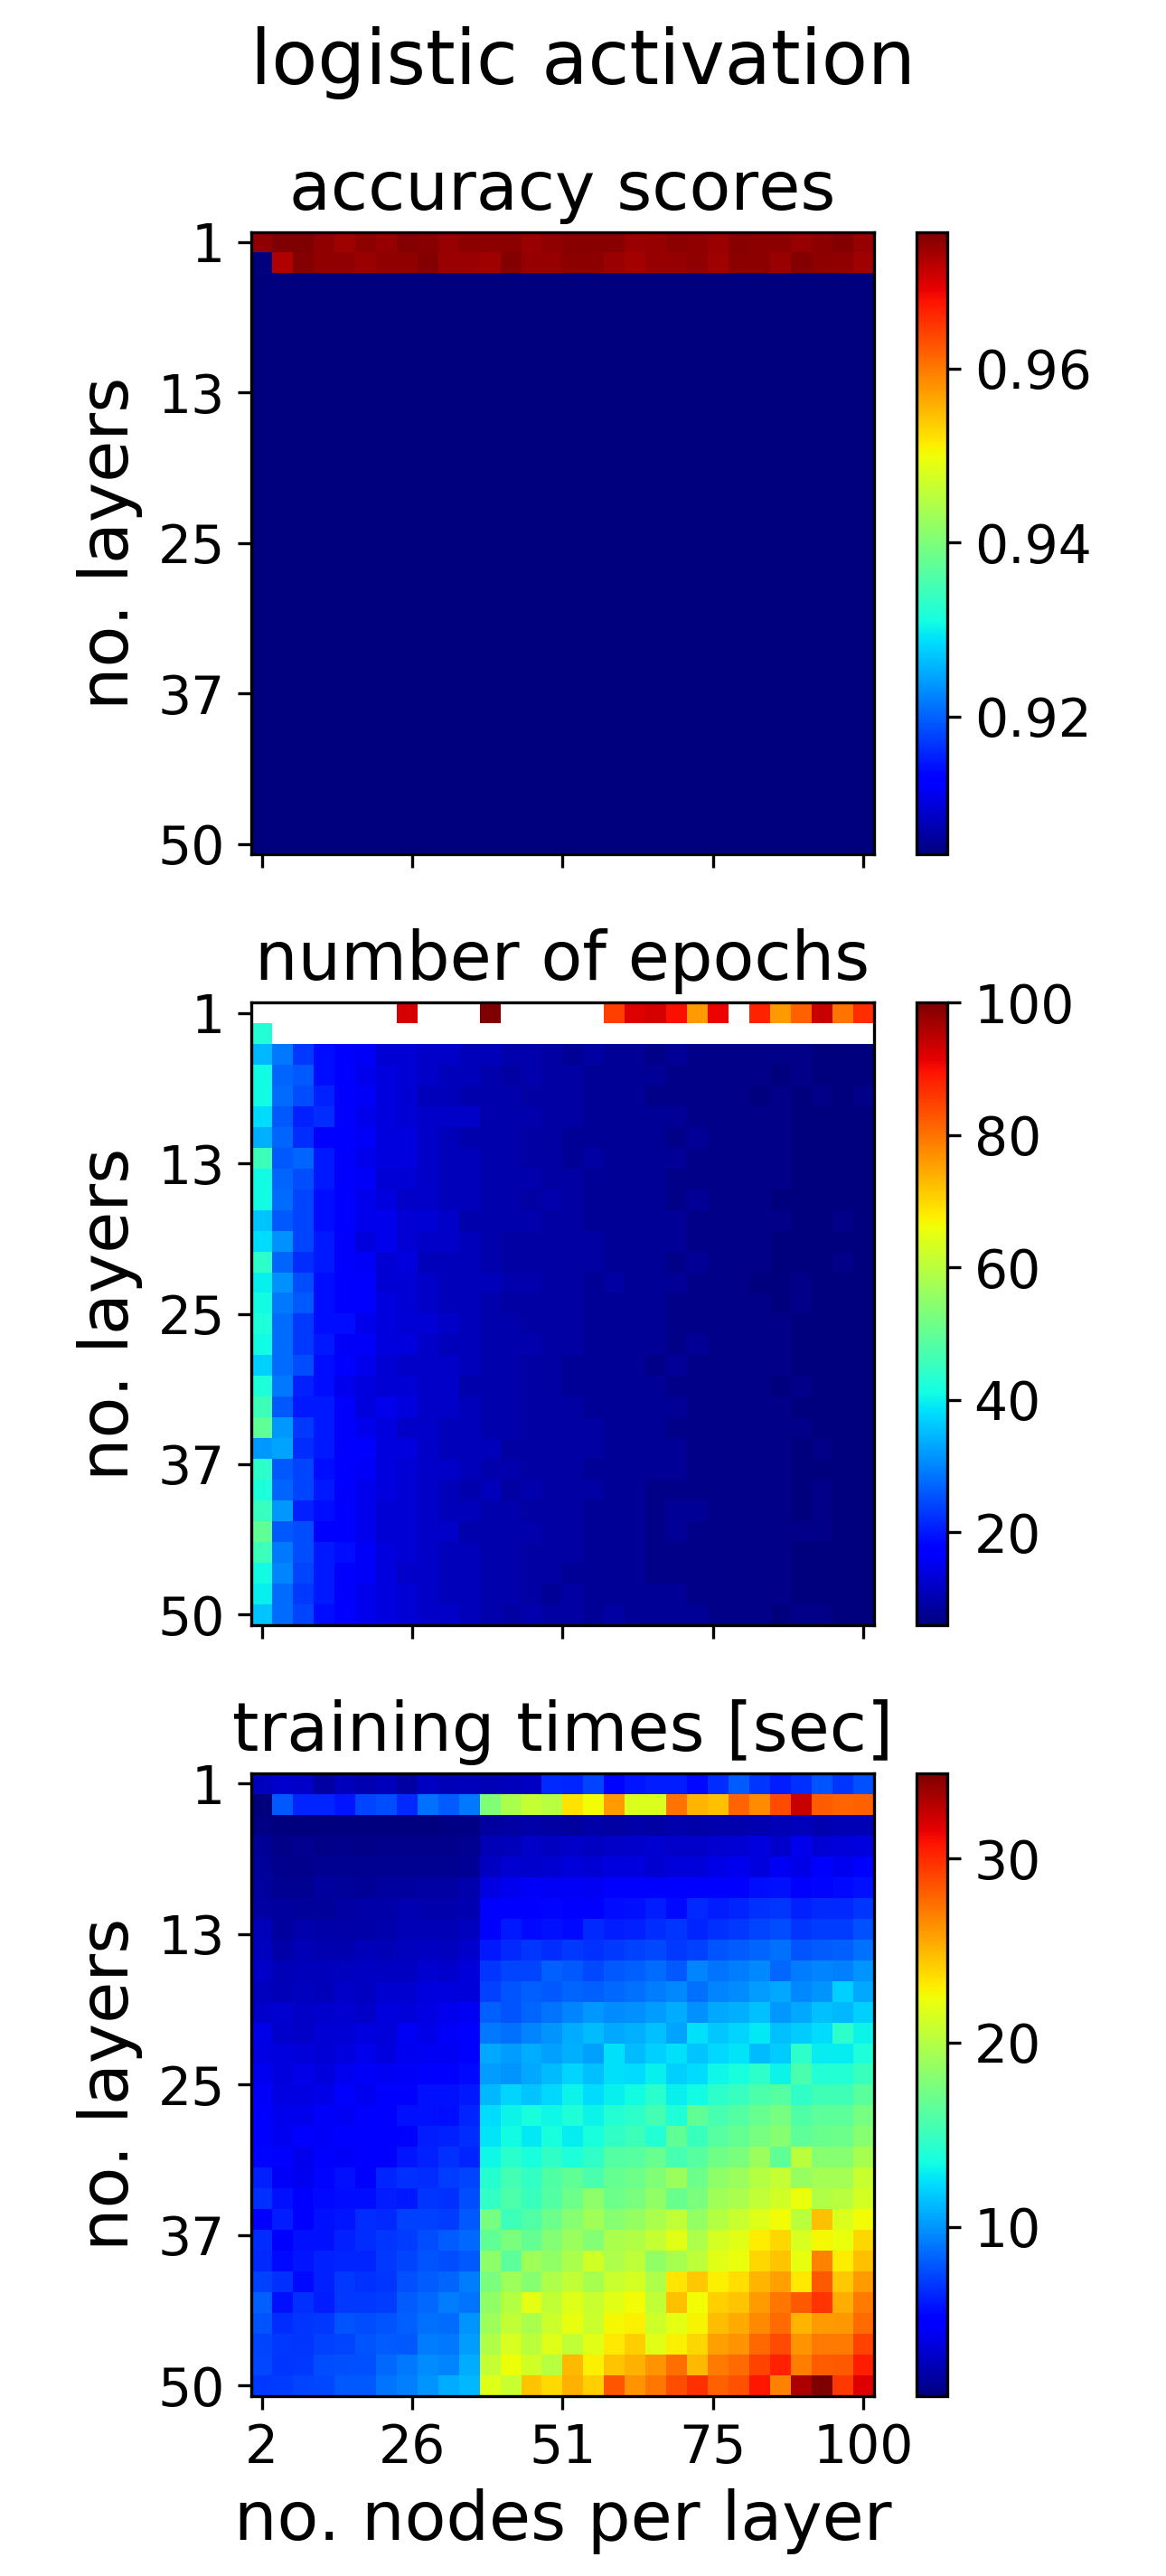
\includegraphics[scale=0.5]{../results/NN/img/gridsearch1_logistic1.png}
	\end{subfigure}
	~
	\begin{subfigure}{0.32\textwidth}
	\centering
	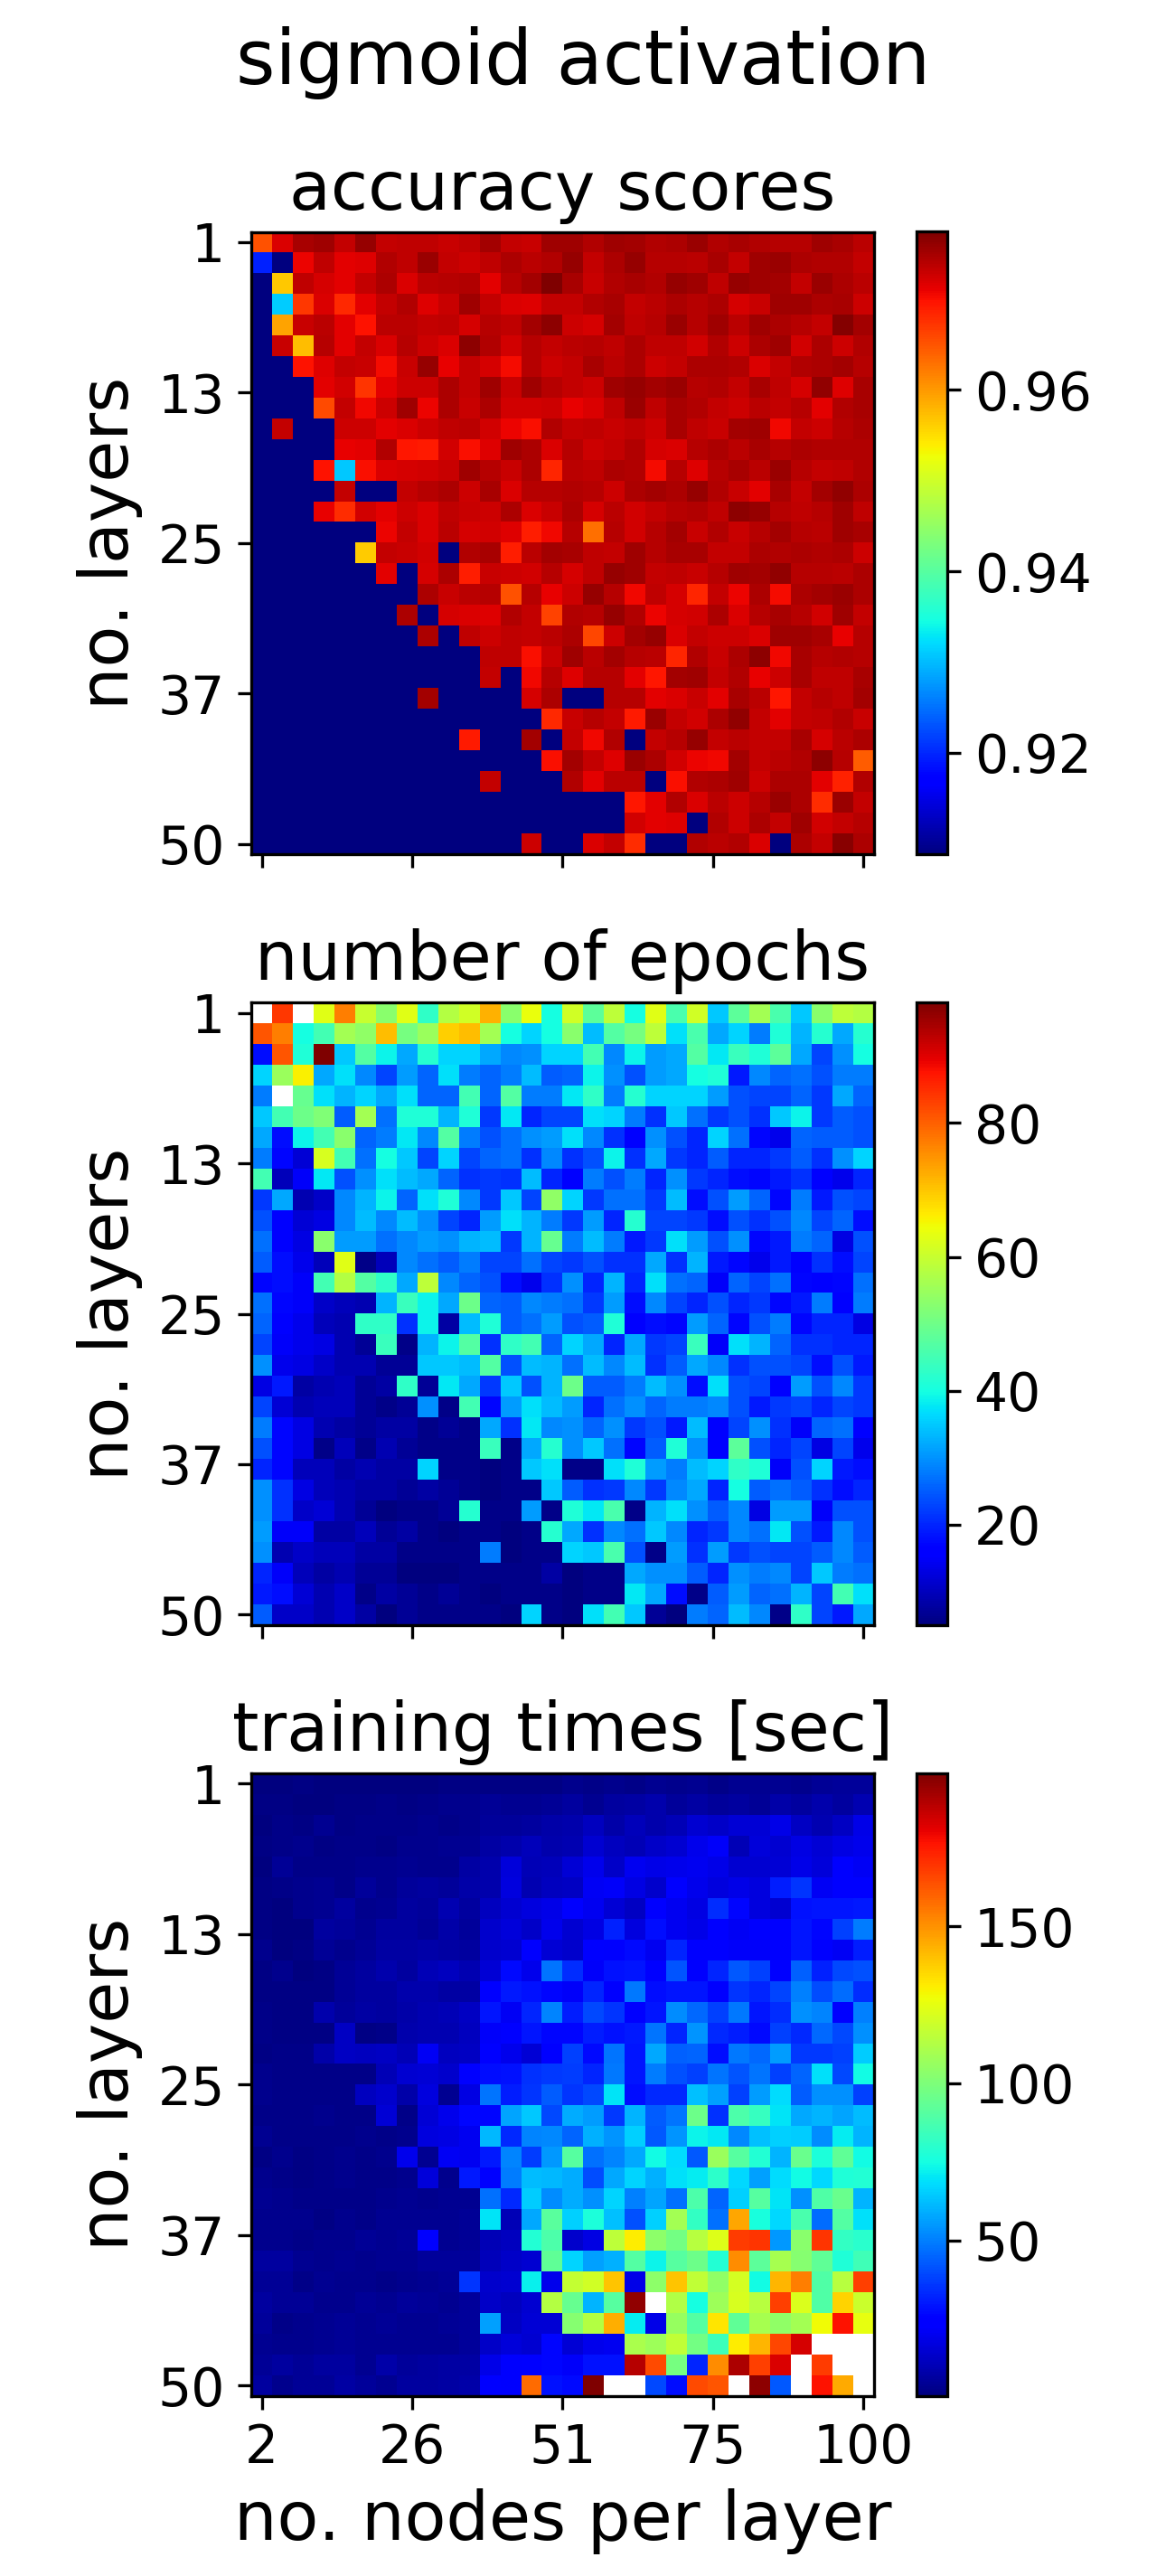
\includegraphics[scale=0.5]{../results/NN/img/gridsearch1_tanh1.png}
	\end{subfigure}
	~
	\begin{subfigure}{0.32\textwidth}
	\centering
	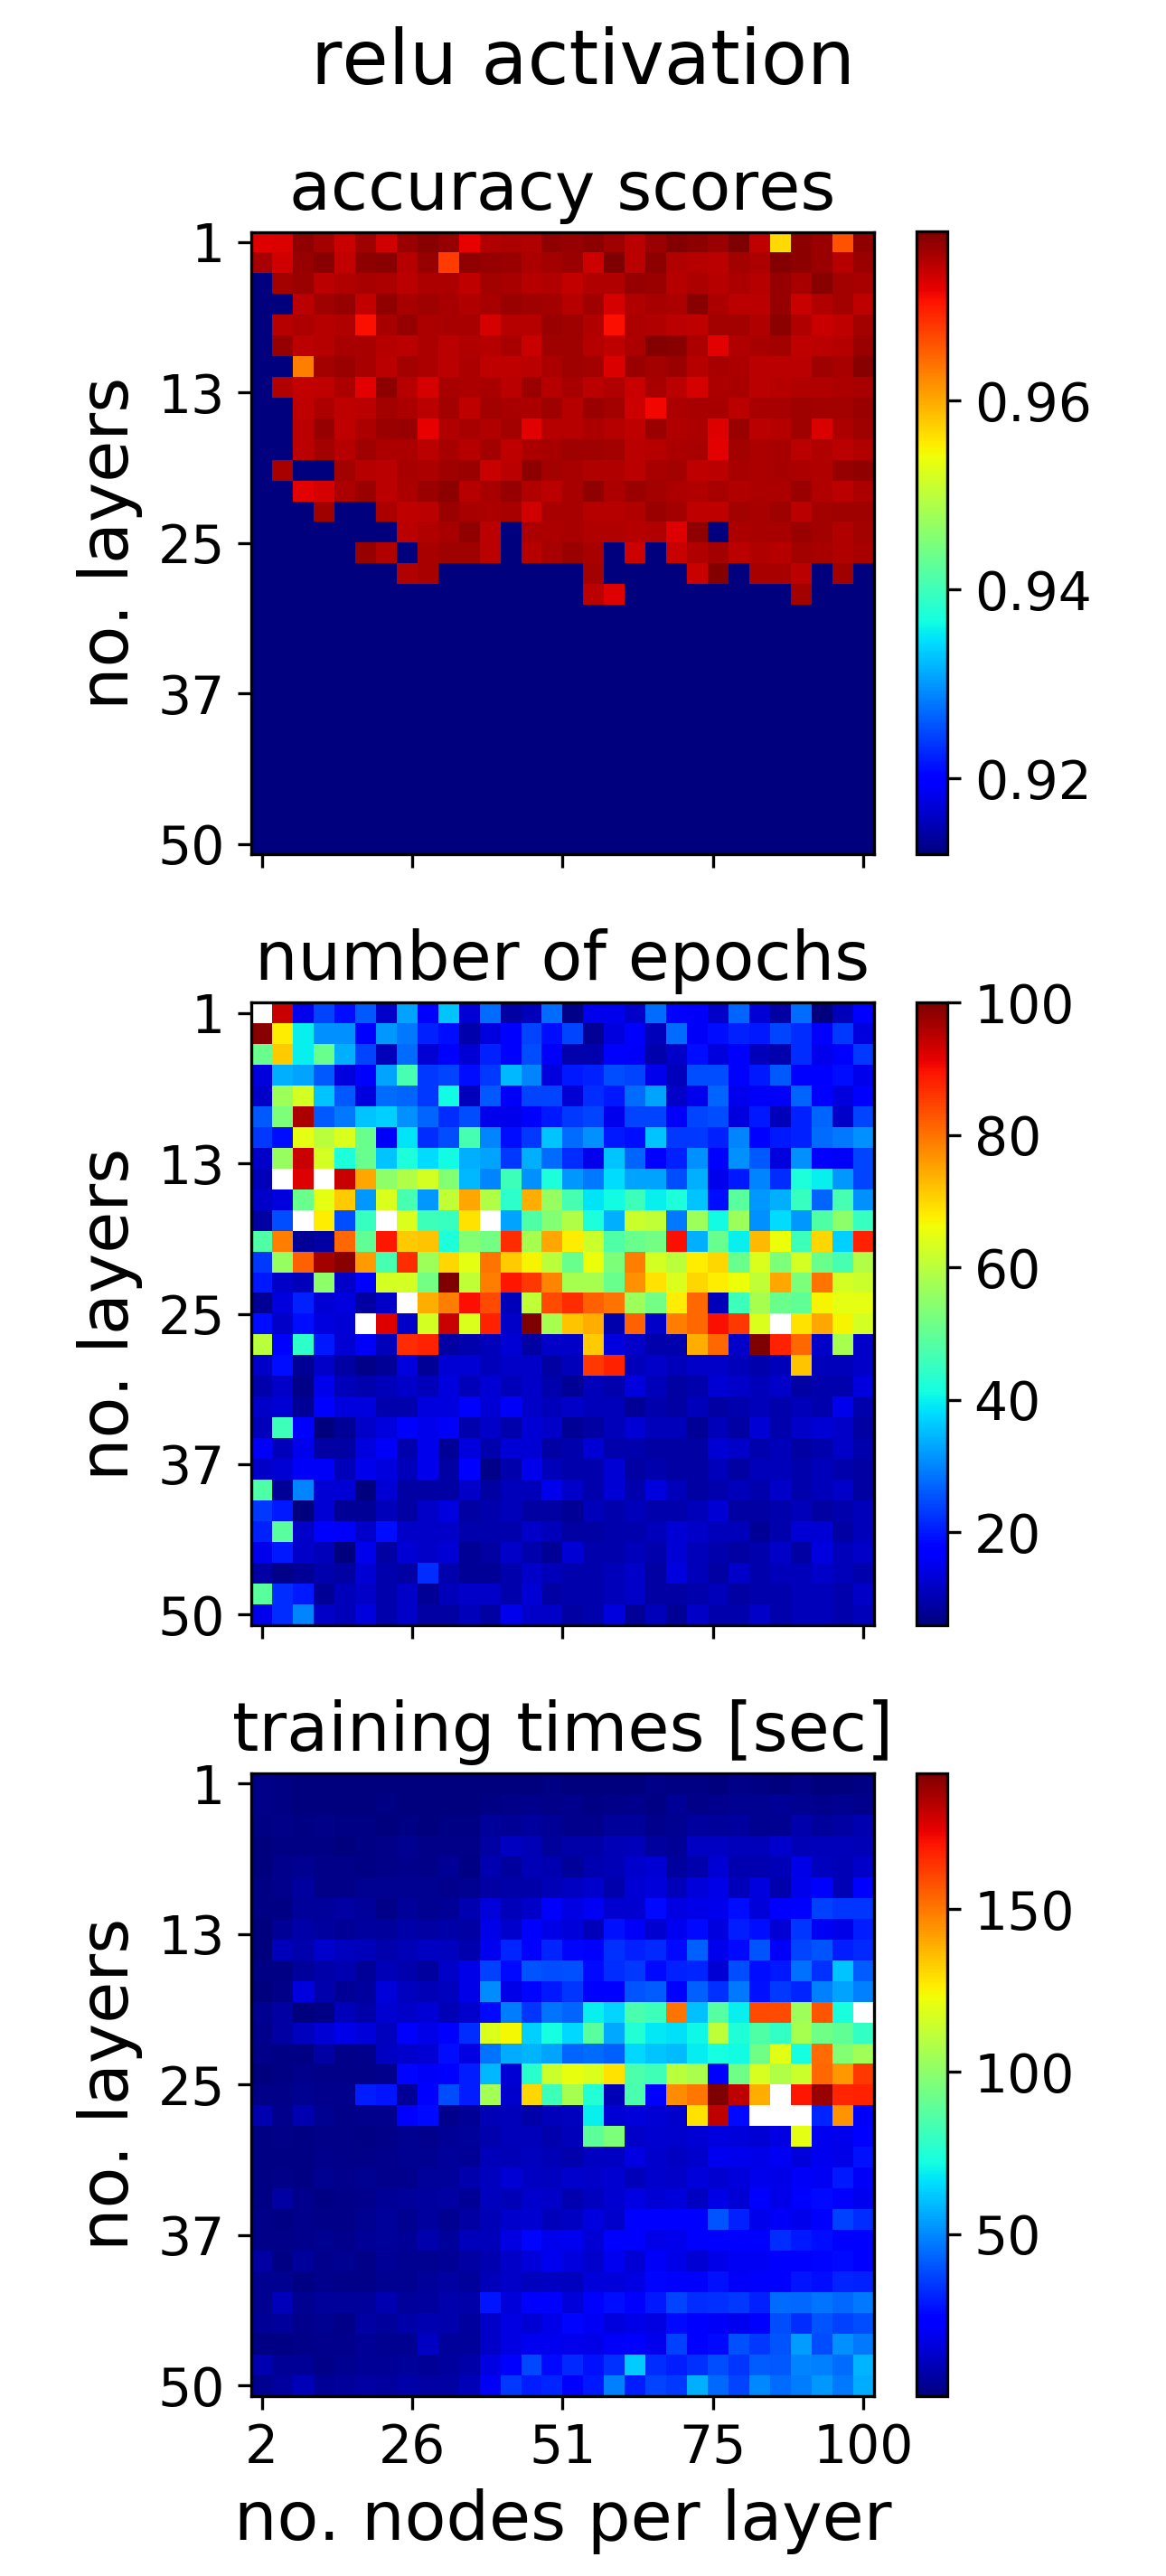
\includegraphics[scale=0.5]{../results/NN/img/gridsearch1_relu1.png}
	\end{subfigure}	
\caption{Hyperparameter analysis of the complexity of neural networks. In general, network complexity increases along the diagonal from the upper left to the lower right. An upper threshold of 150 epochs and 200 seconds is used to focus the colormaps, white pixels have passed the threshold.}
\label{fig:NNgridsearch1}
\end{figure*}

\clearpage
~
\begin{figure*}[h!]
\centering
\begin{subfigure}{0.99\textwidth}
	\begin{subfigure}{0.32\textwidth}
	\centering
	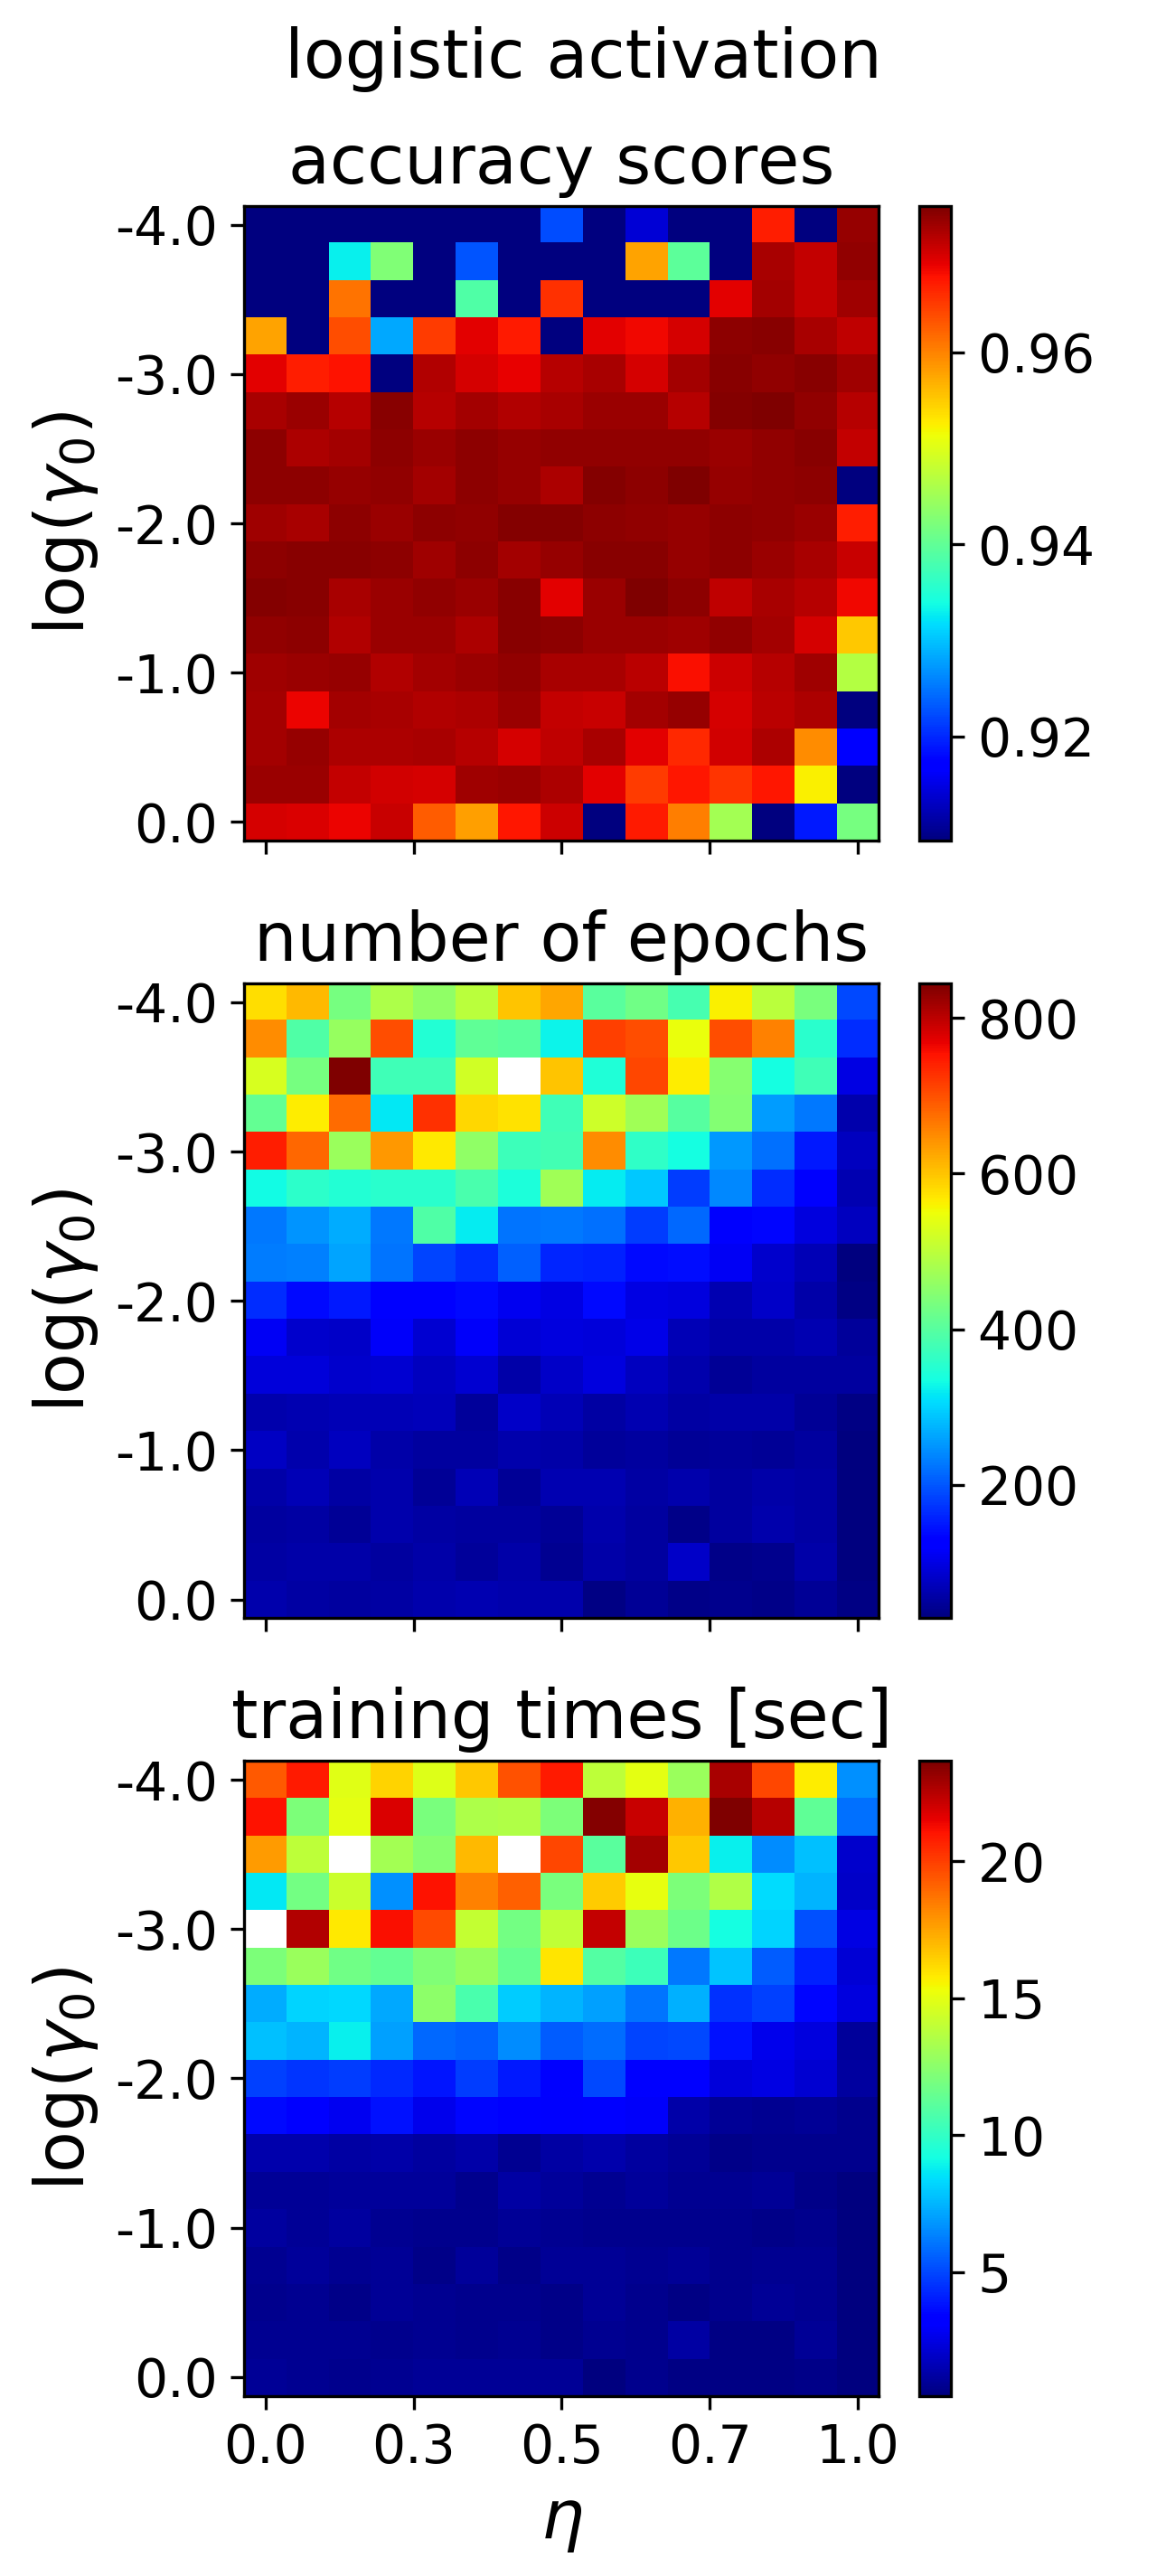
\includegraphics[scale=0.38]{../results/NN/img/gridsearch2_logistic1.png}
	\end{subfigure}
	~
	\begin{subfigure}{0.32\textwidth}
	\centering
	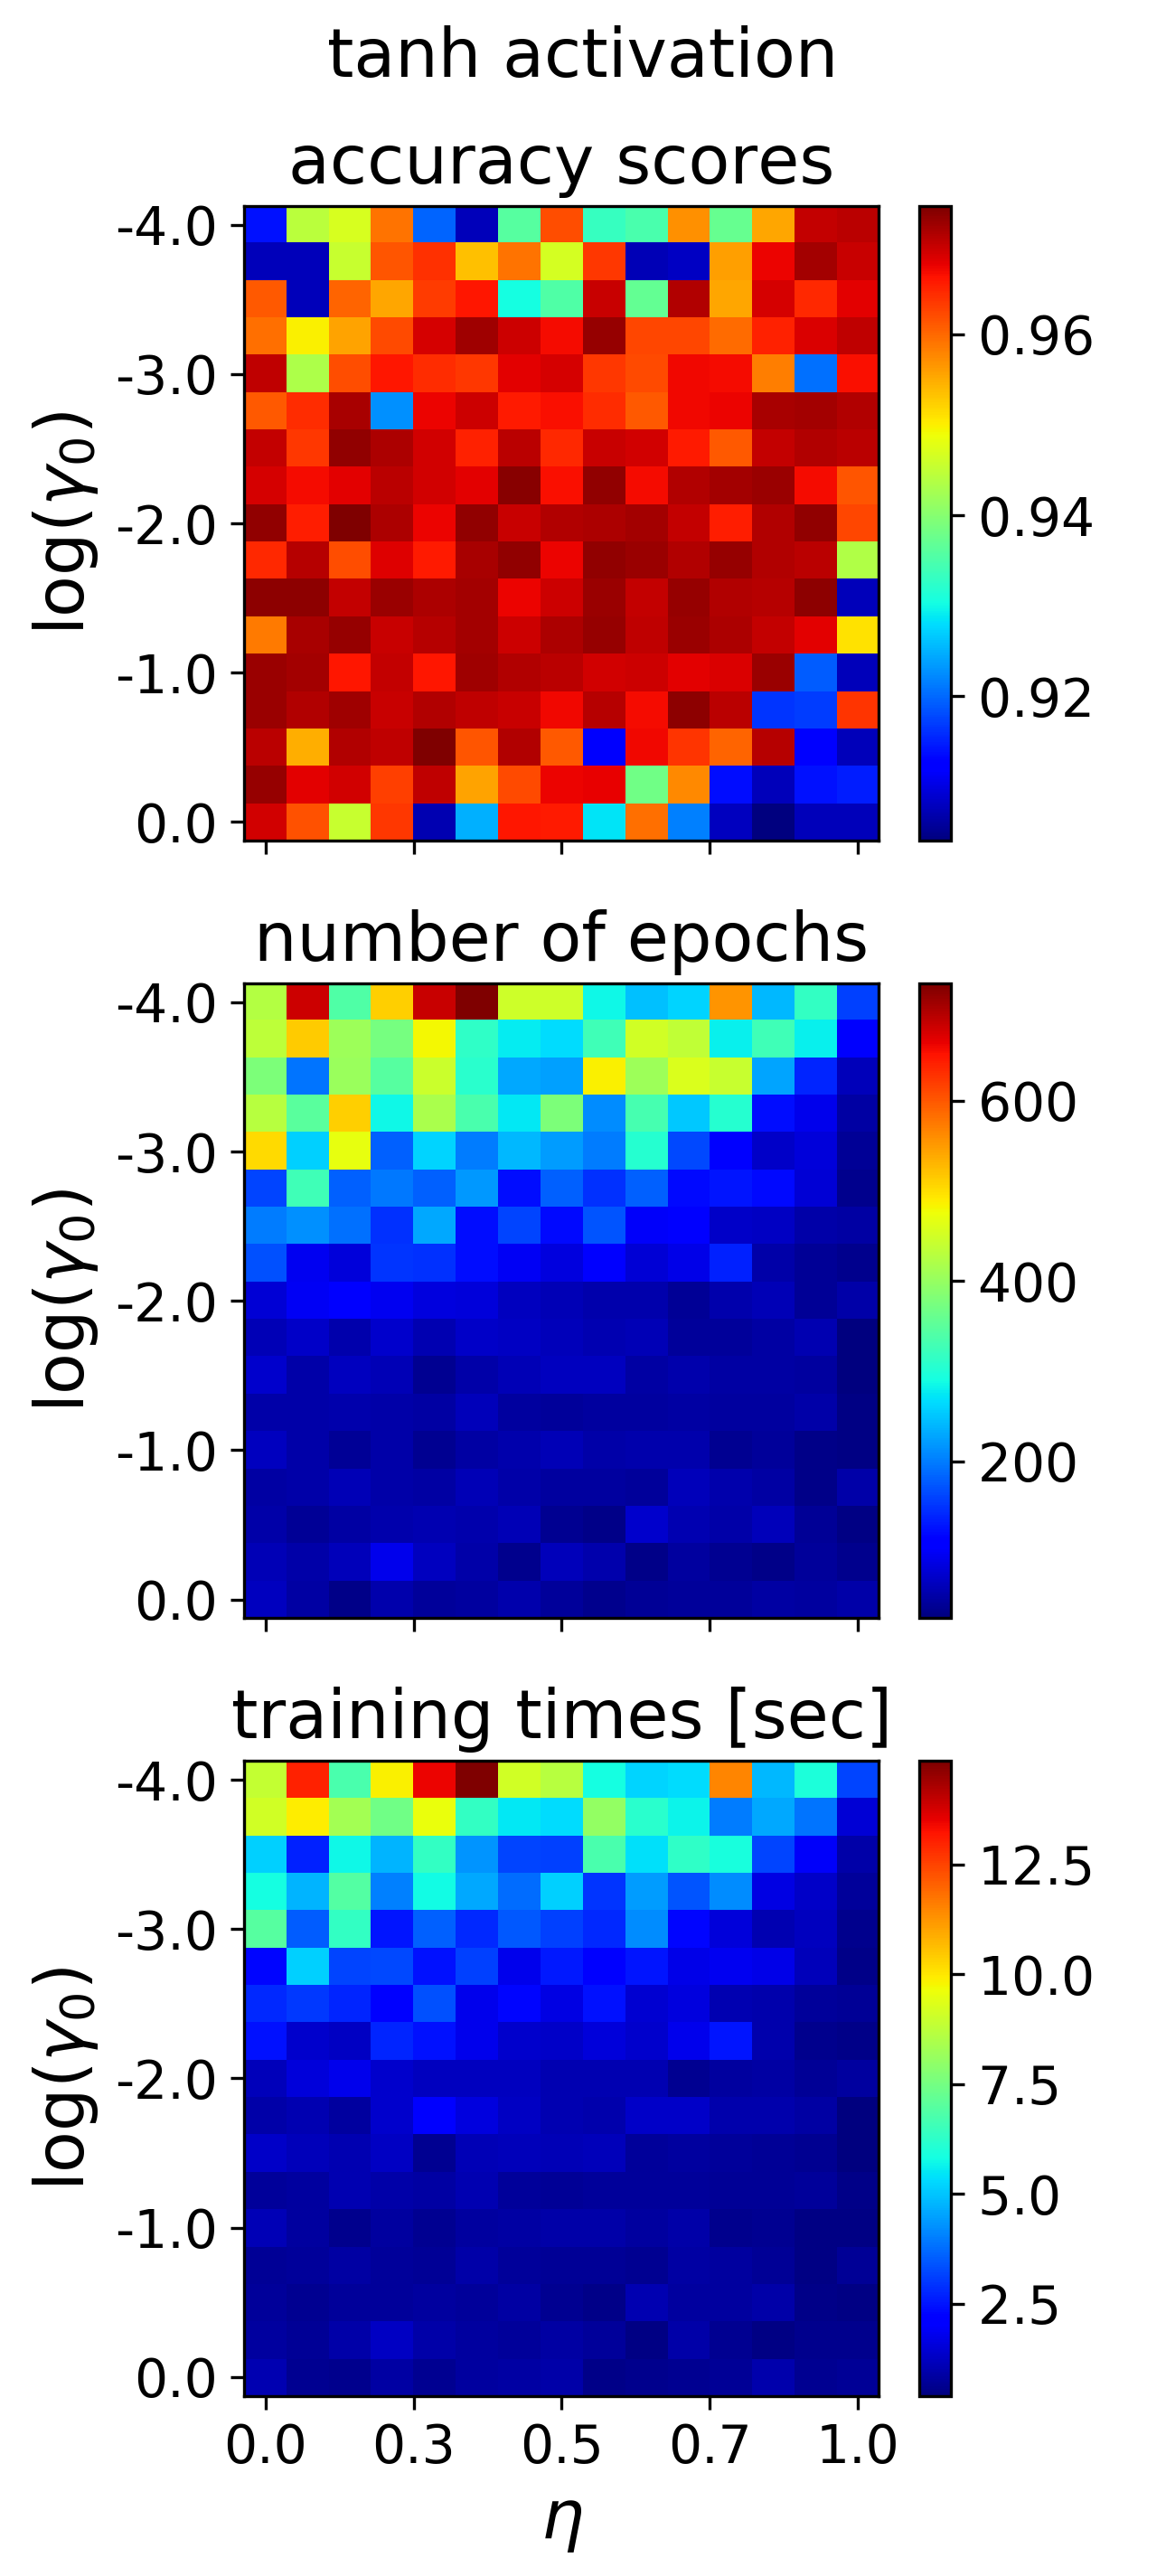
\includegraphics[scale=0.38]{../results/NN/img/gridsearch2_tanh1.png}
	\end{subfigure}
	~
	\begin{subfigure}{0.32\textwidth}
	\centering
	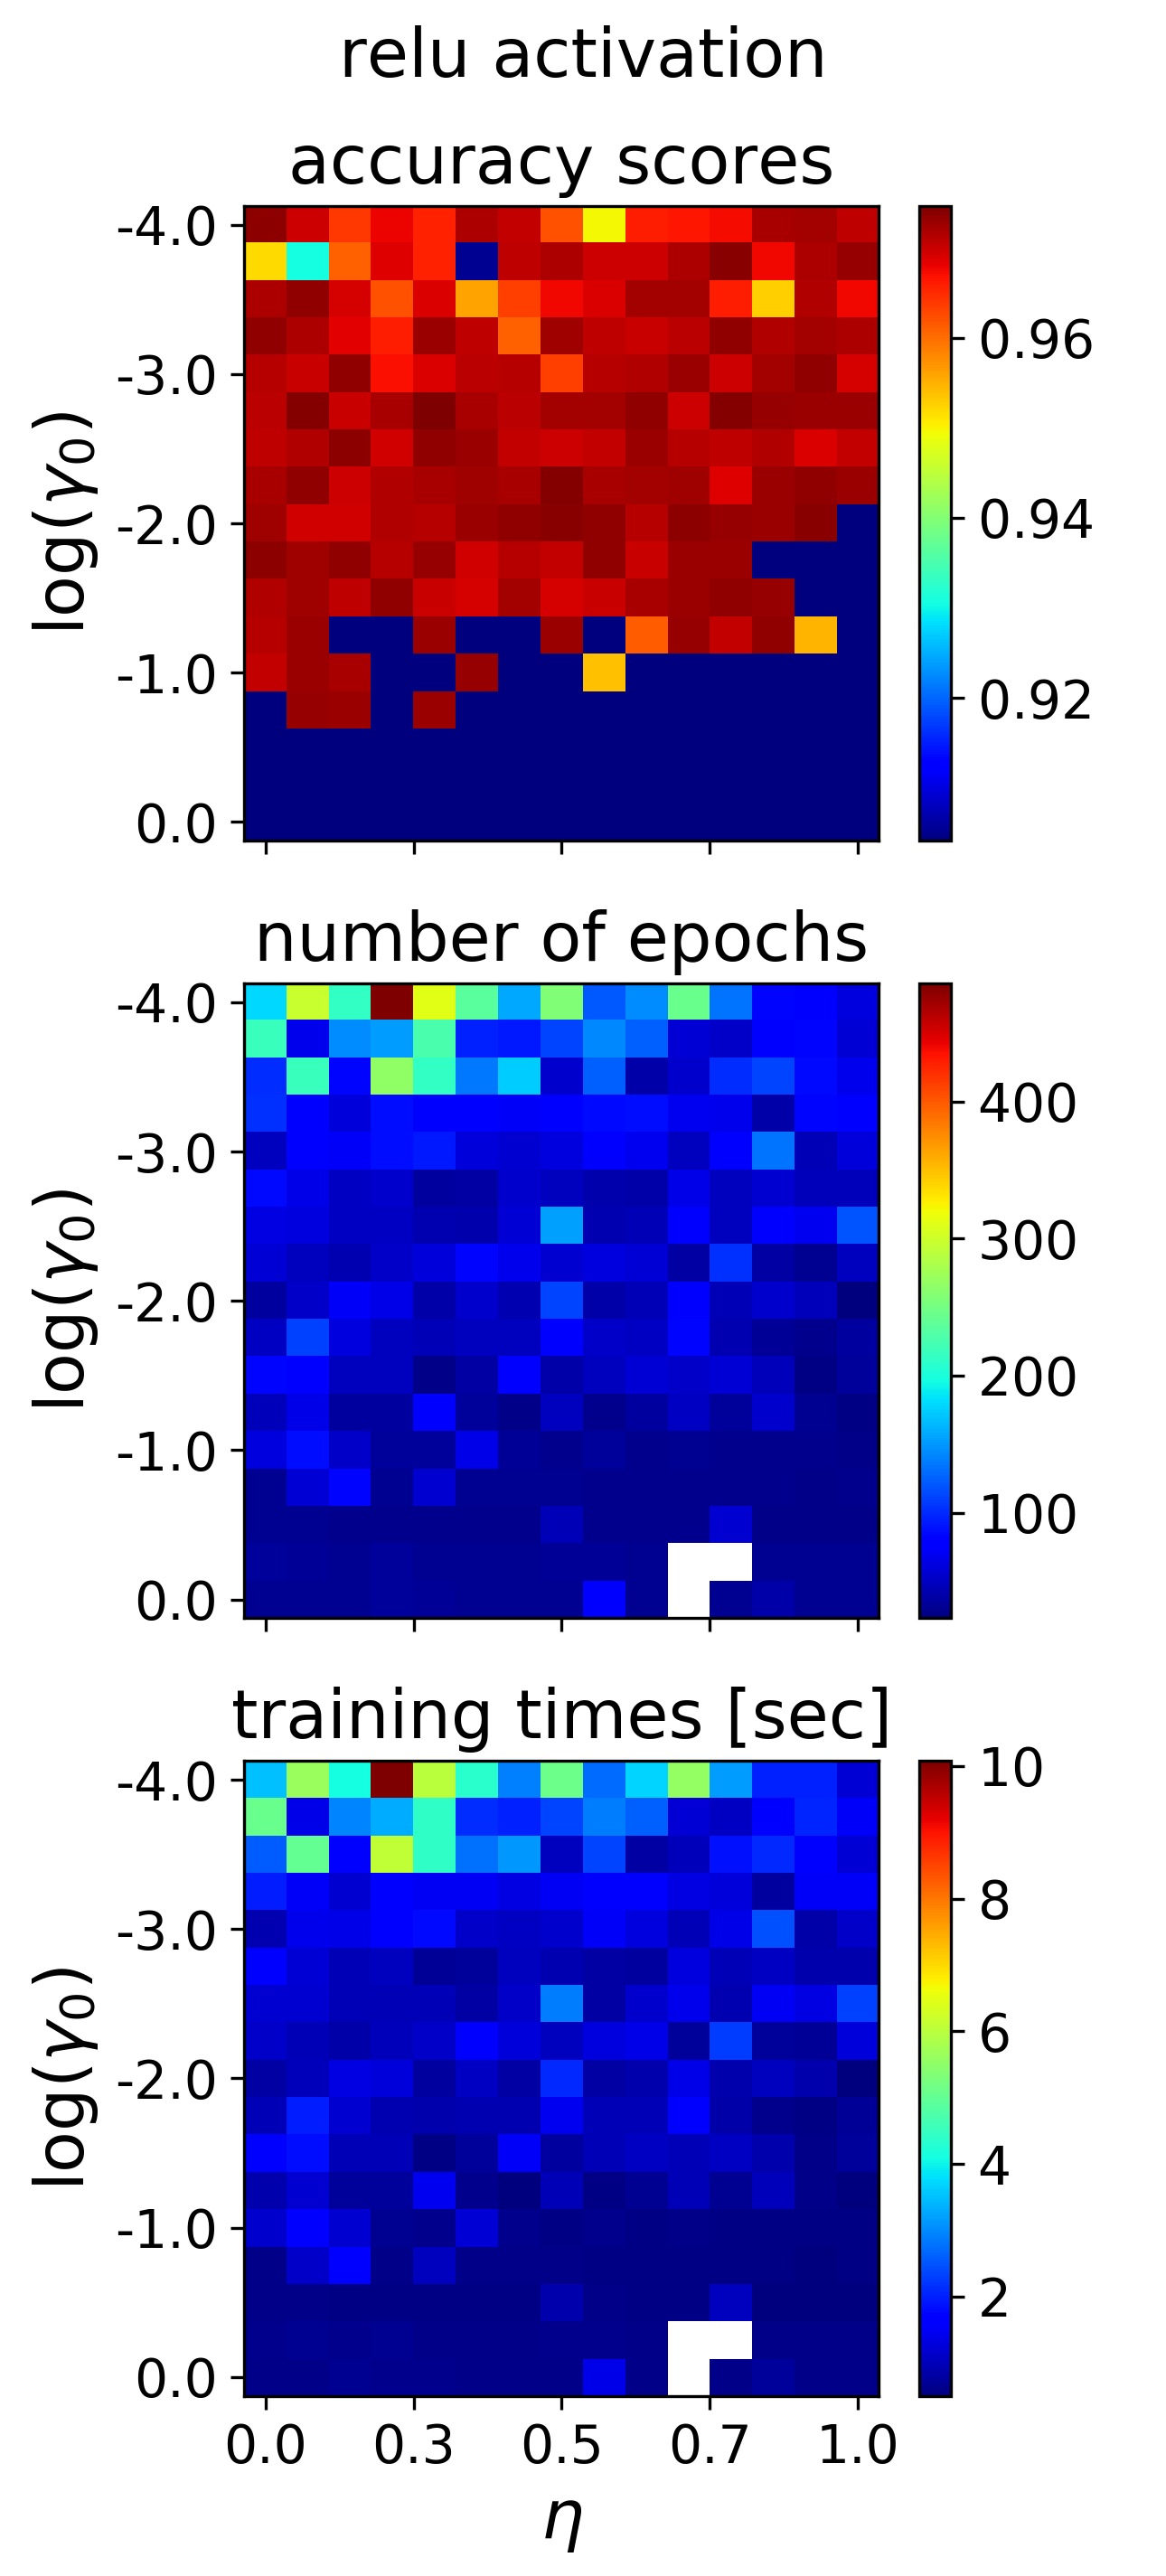
\includegraphics[scale=0.38]{../results/NN/img/gridsearch2_relu1.png}
	\end{subfigure}	
\caption{The simple networks. An upper threshold of 1000 epochs and 25 seconds are used to focus the colormap, white pixels have passed the threshold.}\label{fig:NNgridsearch2_1}
\end{subfigure}
\\[1cm]
\begin{subfigure}{0.99\textwidth}
	\begin{subfigure}{0.32\textwidth}
	\centering
	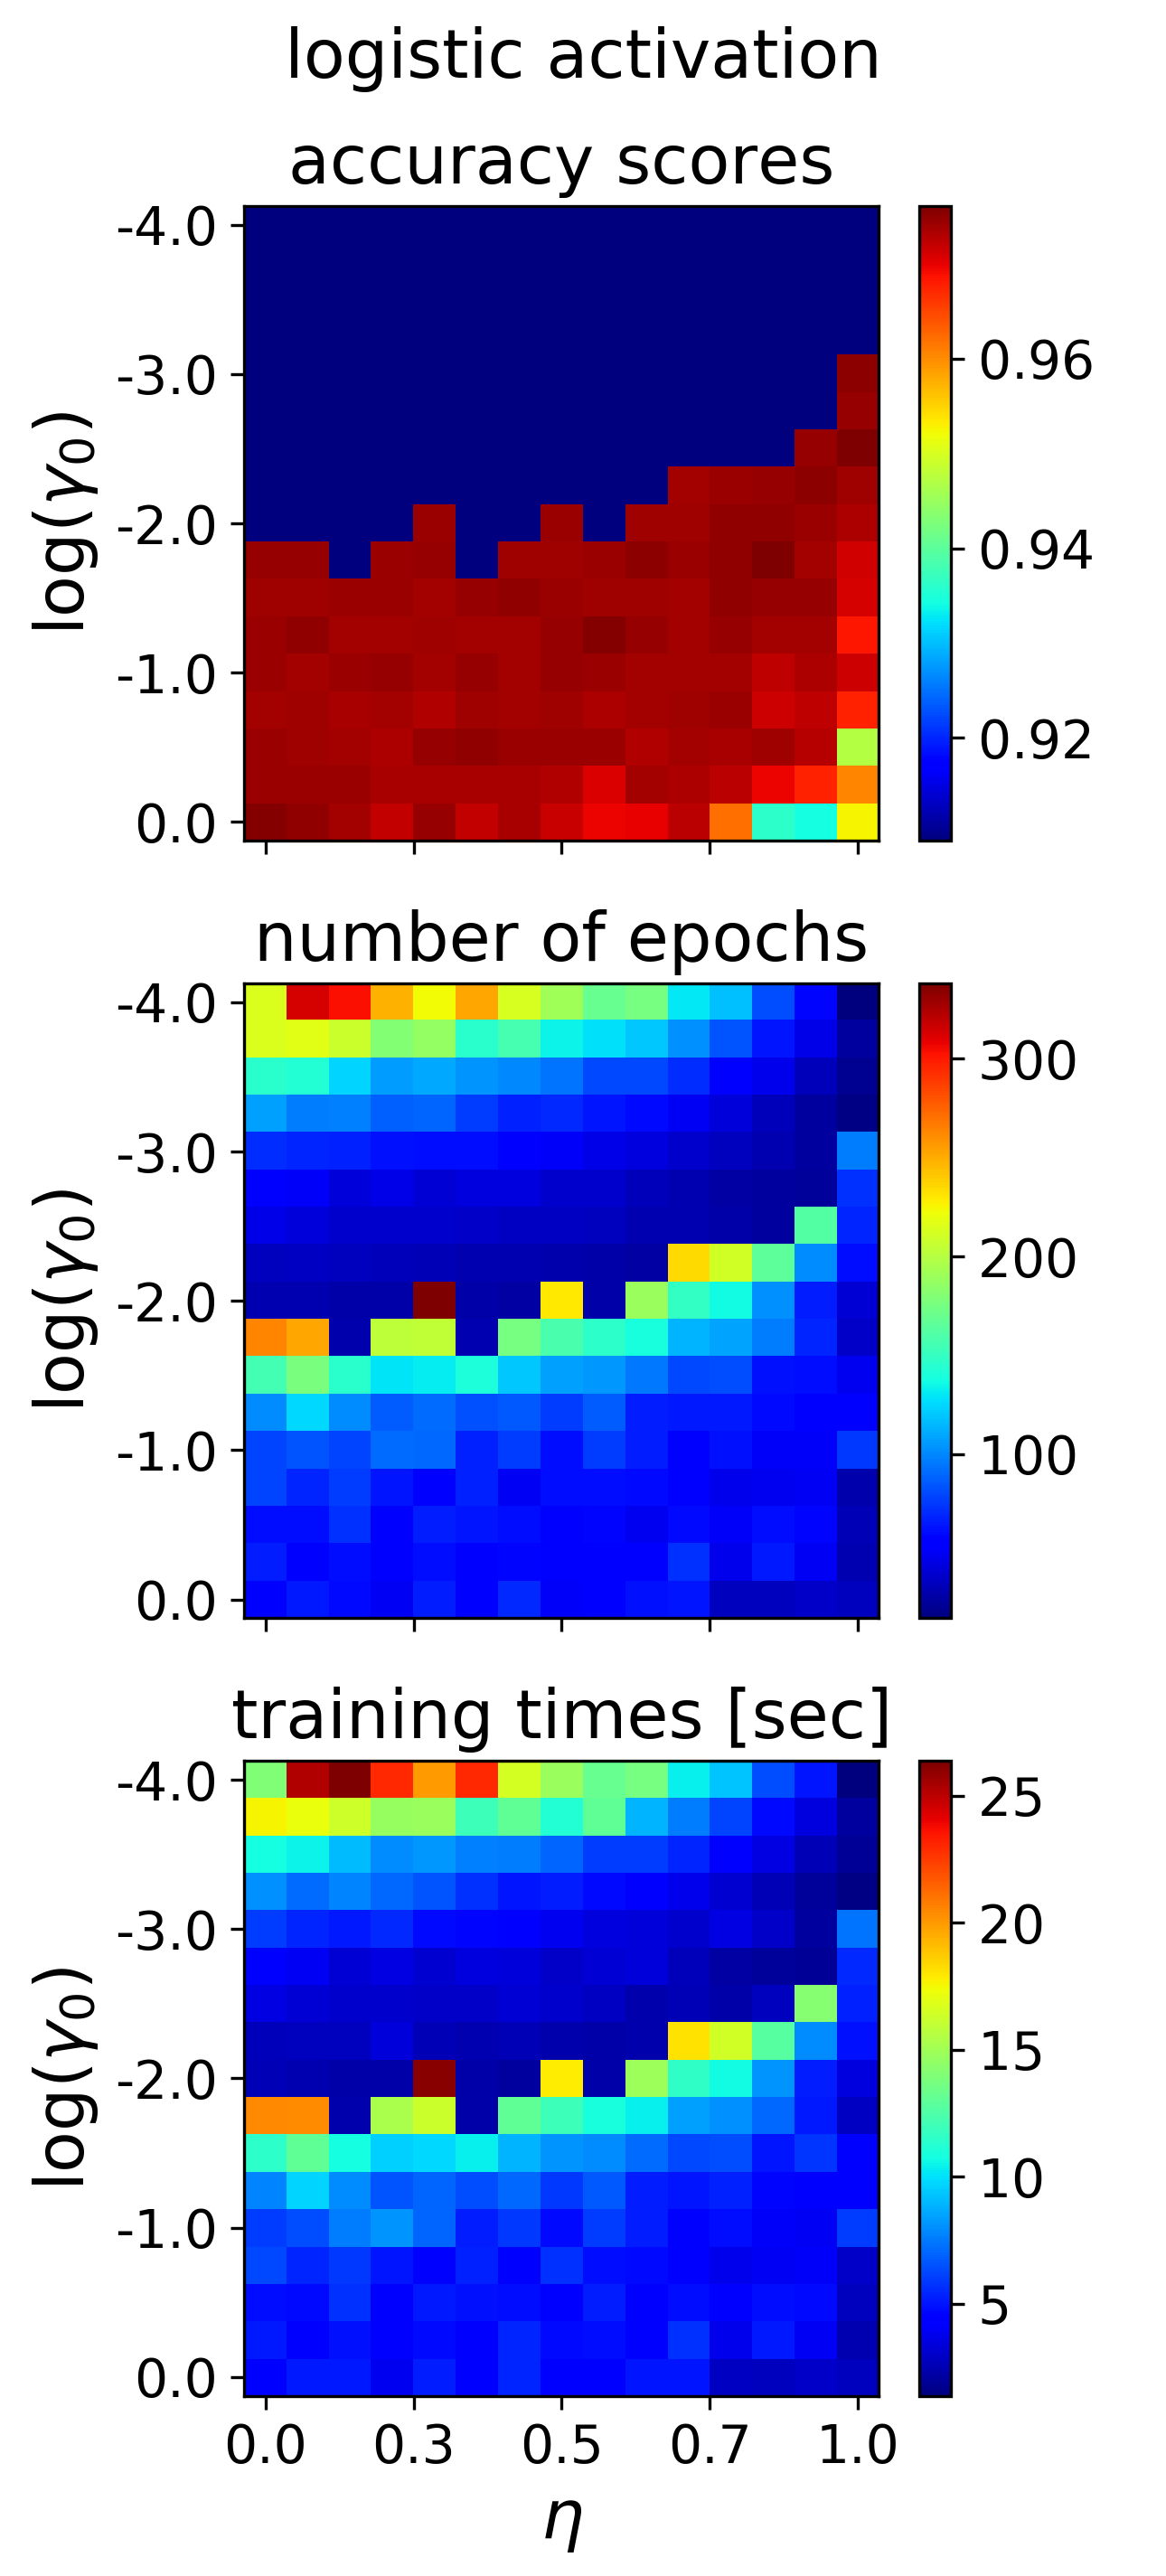
\includegraphics[scale=0.38]{../results/NN/img/gridsearch2_logistic3.png}
	\end{subfigure}
	~
	\begin{subfigure}{0.32\textwidth}
	\centering
	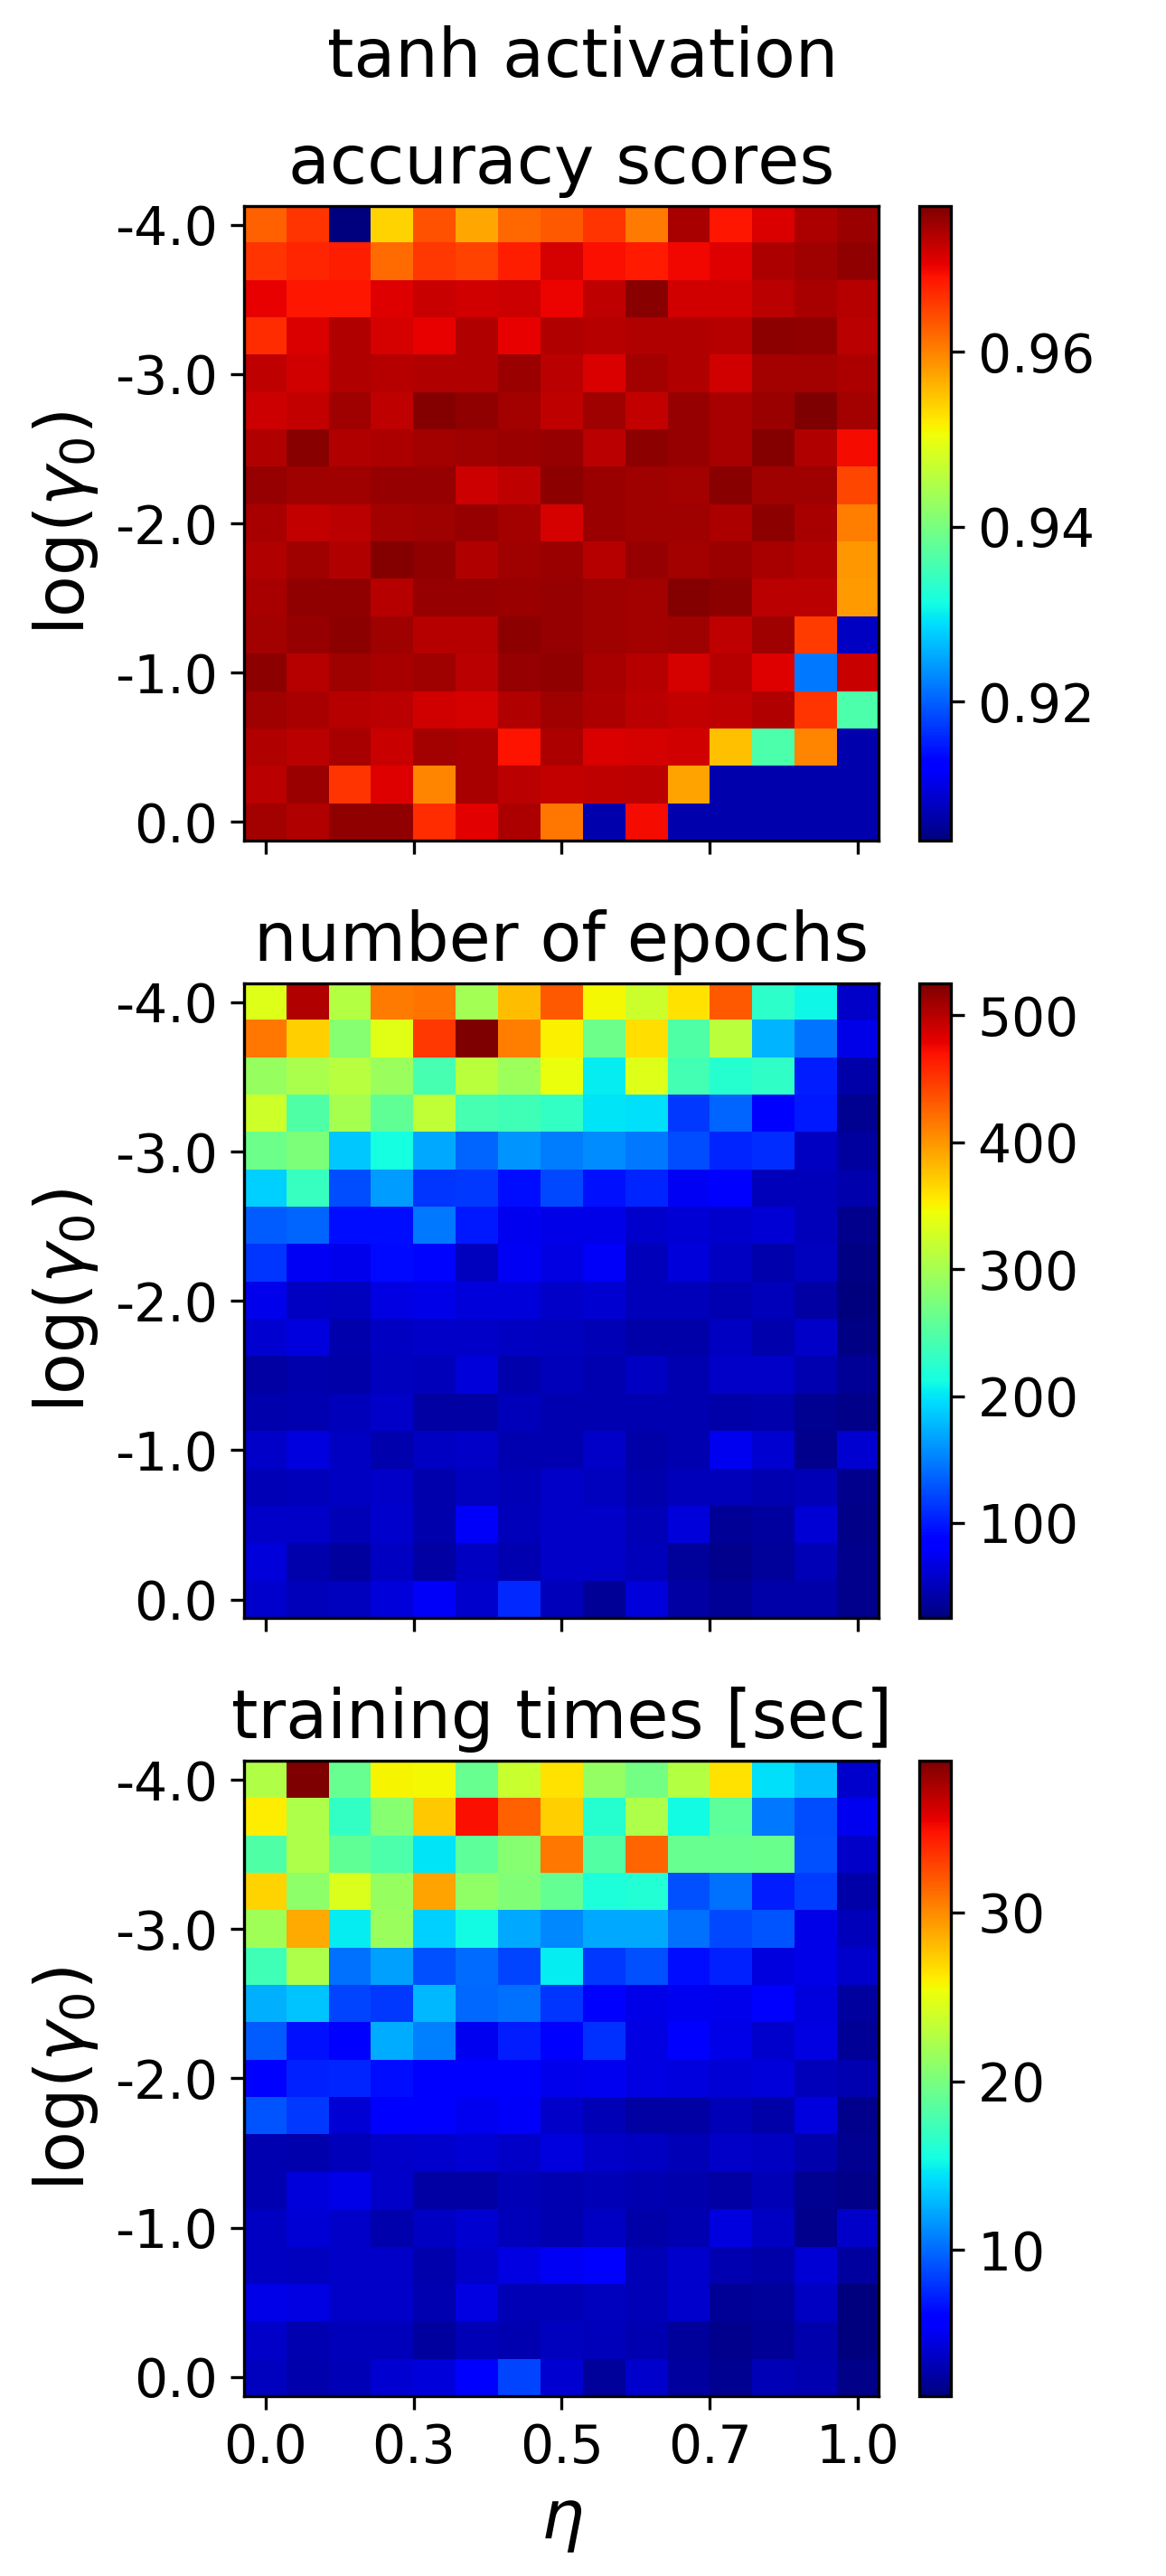
\includegraphics[scale=0.38]{../results/NN/img/gridsearch2_tanh3.png}
	\end{subfigure}
	~
	\begin{subfigure}{0.32\textwidth}
	\centering
	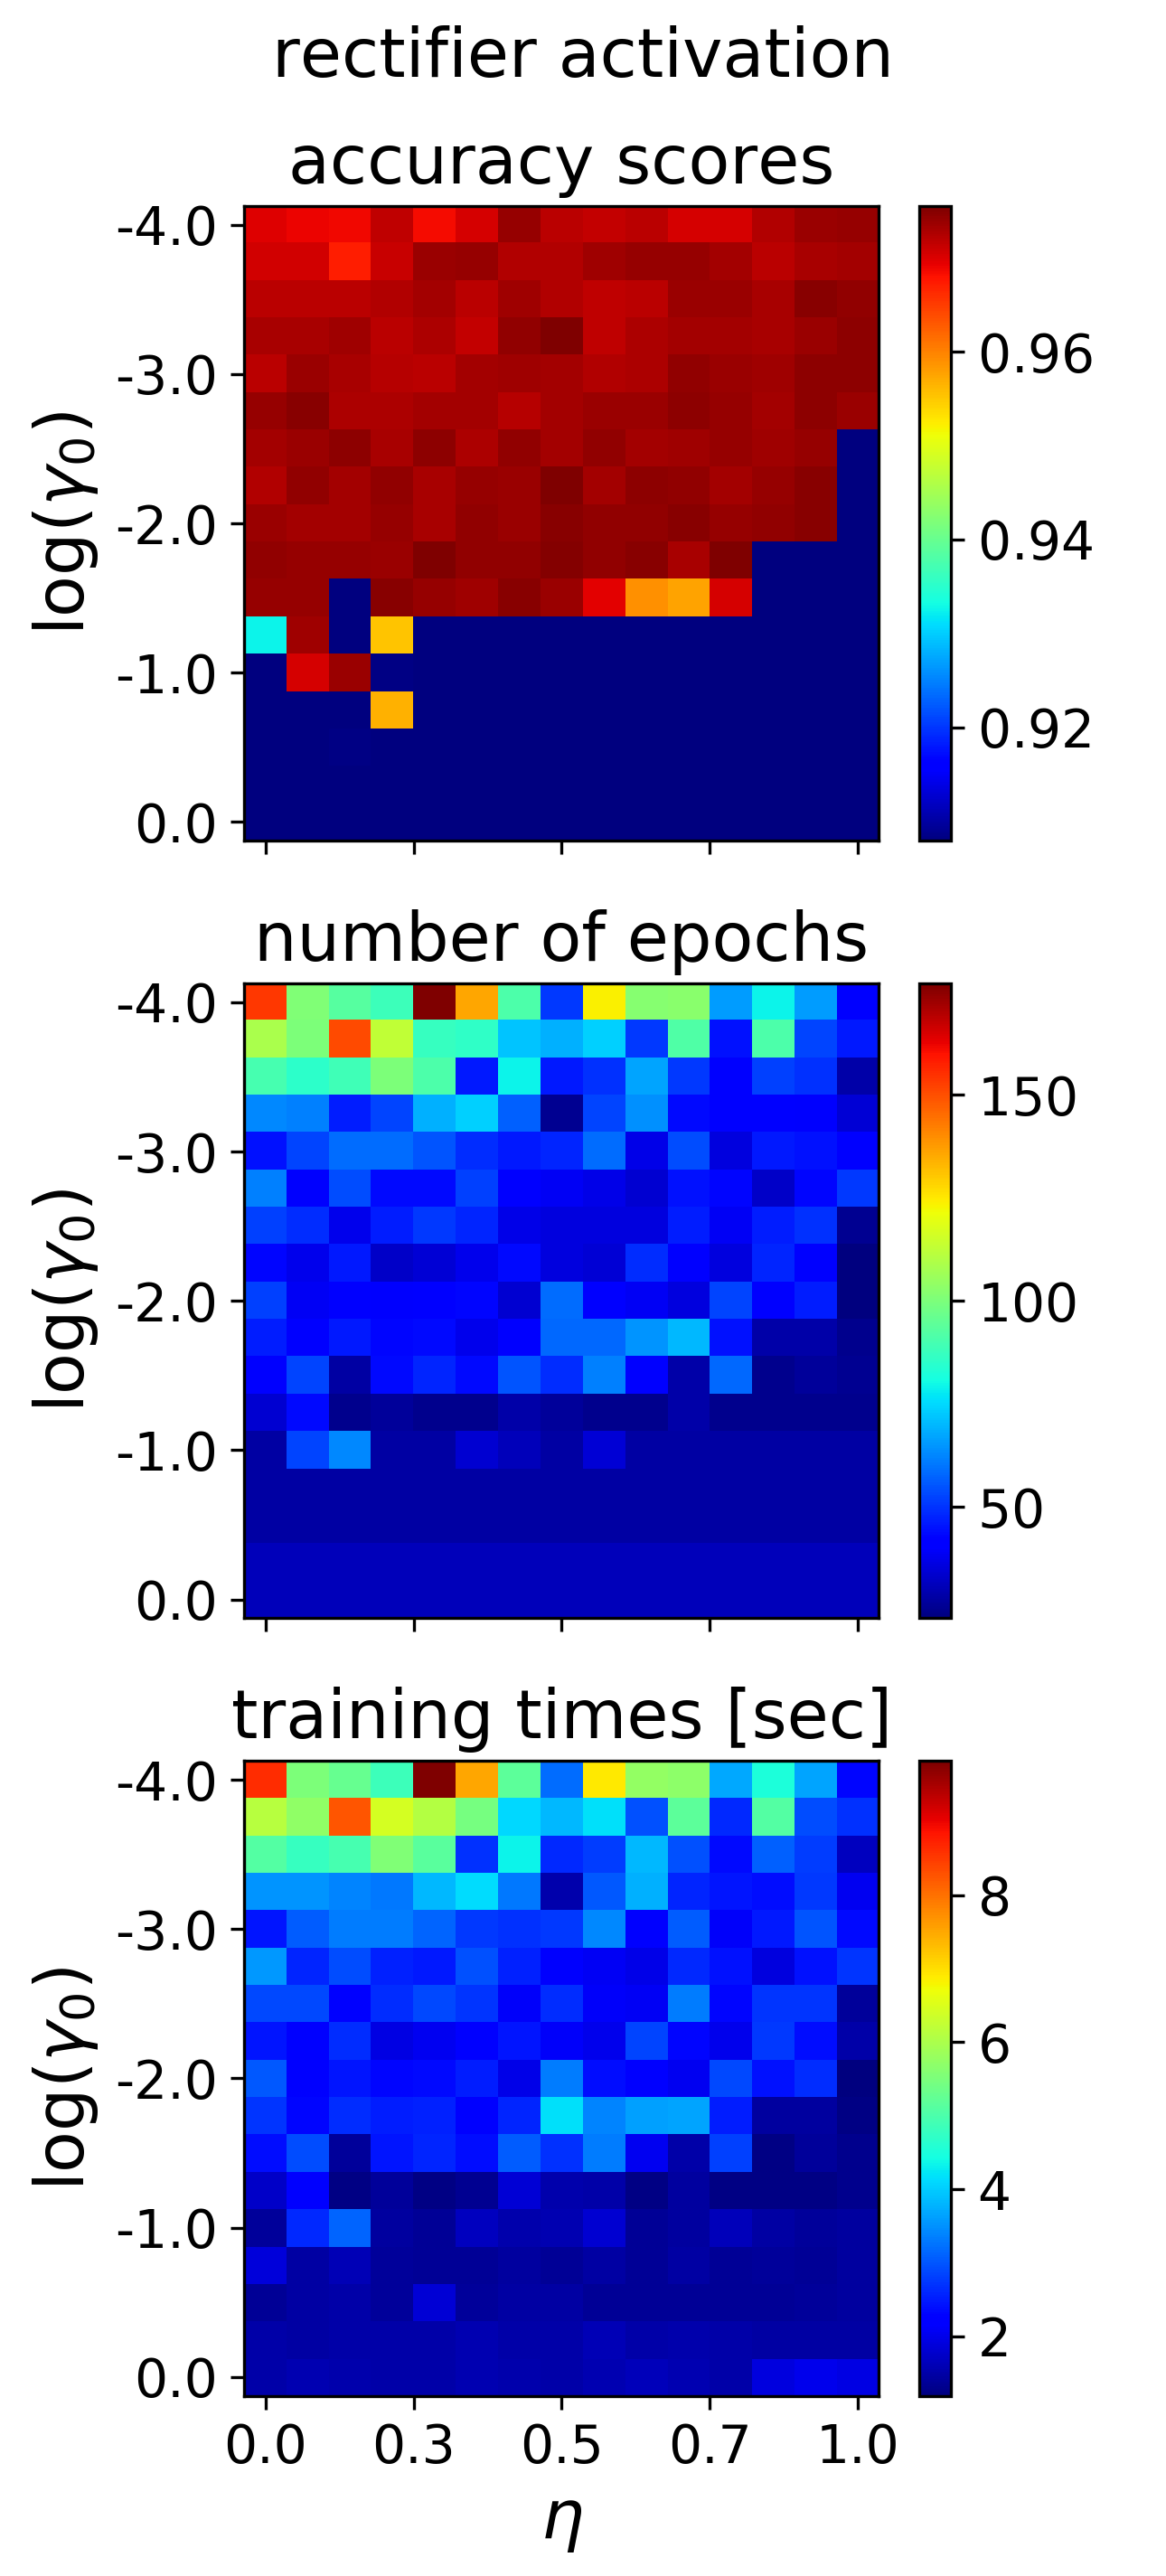
\includegraphics[scale=0.38]{../results/NN/img/gridsearch2_relu3.png}
	\end{subfigure}	
\caption{The complex networks.}\label{fig:NNgridsearch2_2}
\end{subfigure}
\caption{Hyperparameter analysis of the learning scheme of neural networks. As a general rule, the learning rate increases along the diagonal from the upper left to the lower right.}\label{fig:NNgridsearch2}
\end{figure*}
\clearpage

\begin{figure*}
\centering
	\begin{subfigure}{0.48\textwidth}
	\centering
	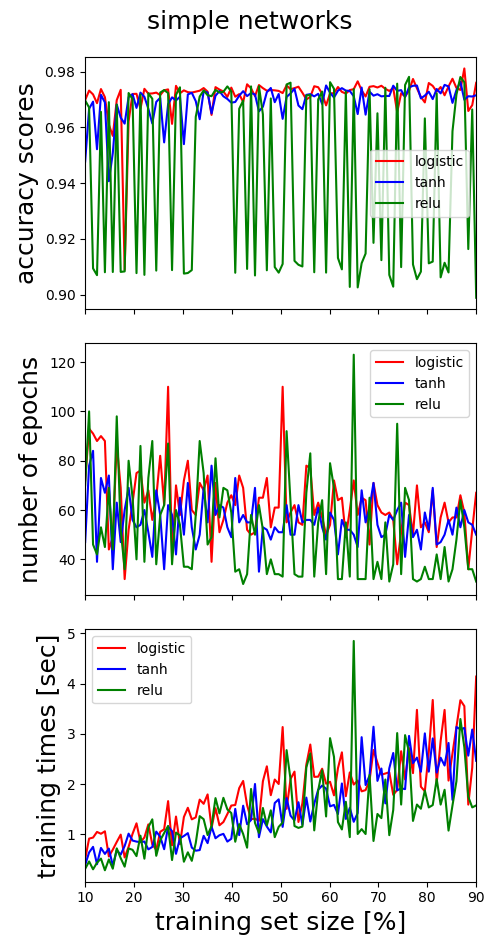
\includegraphics[scale=0.45]{../results/NN/img/gridsearch3_1_8_1.png}
	\caption{Simple networks, trained with \(\gamma_0=10^{-1}\) and \(\eta=0.3\).}
	\label{fig:NNgridsearch3_simple}
	\end{subfigure}
	~
	\begin{subfigure}{0.48\textwidth}
	\centering
	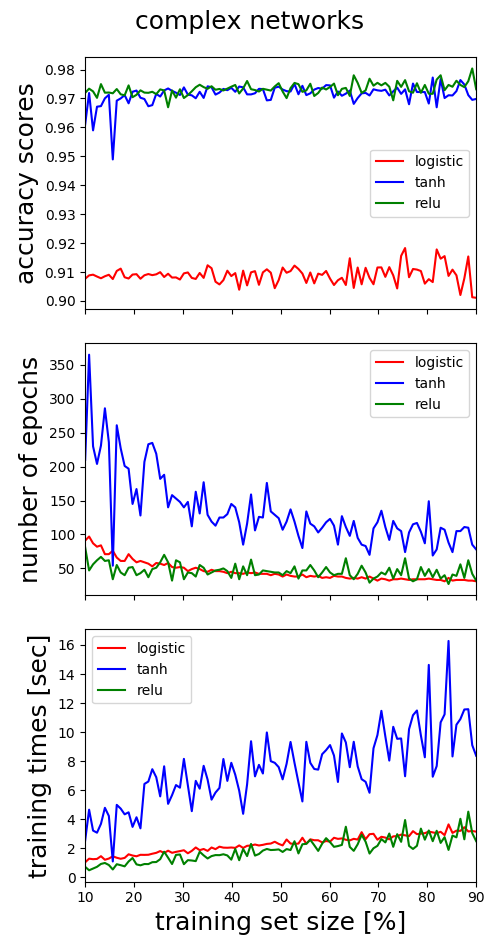
\includegraphics[scale=0.45]{../results/NN/img/gridsearch3_3_30_3.png}
	\caption{Complex networks, trained with \(\gamma_0=10^{-3}\) and \(\eta=0.7\).}
	\label{fig:NNgridsearch3_complex}
	\end{subfigure}
\caption{Hyperparameter analysis of training set size's impact on neural networks overfitting.}
\label{fig:NNgridsearch3}
\end{figure*}

\twocolumngrid

\subsubsection{Training set overfitting}
The overfitting analysis was run for all network activations, for both simple and complex network structures, and for each of the three learning parameter sets from the training scheme analysis. Much of the results highlight the same relationships, as well as reiterate the results of the previous analysis. To avoid uneccessary figures, only two plots have been included: the analysis using simple networks, trained with \((\gamma_0,\eta)=(10^{-1},0.3)\), and the analysis using complex networks, trained with \((\gamma_0,\eta)=(10^{-3},0.7)\). The rest of the material, together with some additional material using different network structures, is included in the GitHub repository. The main results of the analysis are shown in figure \ref{fig:NNgridsearch3}.

Quite unexpectedly, the training set sizes have almost no impact on the network accuracies. Nevertheless, some data results do show a slight decrease in accuracy with training set sizes less than 20\%. In addition, some networks' accuracies become less stable with increased training set sizes, e.g. the logistic networks in figure \ref{fig:NNgridsearch3_complex}. This could suggest some minor overfitting, however the resulting variations in the accuracy scores are miniscule compared the difference between the low and high accuracy regions seen in previous analyses.

Seeing that \((\gamma_0,\eta)=(10^{-1},0.3)\) is just on the low-to-high accuracy boundary for the rectifier networks (see figure \ref{fig:NNgridsearch2}), the unstable behaviour of the rectifier networks in figure \ref{fig:NNgridsearch3_complex} comes as no surprise. The erratic behaviour seems to be uniformly spread, suggesting whether a nerual network falls within the low or accuracy regions boils down to chance. This hypothesis is further supported by the fact that the neural network's weights and biases have random initial conditions. There does not seem to be any clear mechanisms with which such a strict boundary should appear (as opposed to smooth boundary), other than its a peculiarity of the BPA algorithm itself.

Furthermore, there is a general trend for training time to increase with increasing training set size, but this is expected. Especially in the case of the simple networks, which are more or less the same for all network activations. However, in the case of the complex networks, the sigmoid networks require a much larger numer of epochs, and thus time, to train. Despite this however, the sigmoid networks have no accuracy benefit over the rectifier networks (that is, in figure \ref{fig:NNgridsearch3_complex}).

It is clear that the training set size need not be greater than say 20\%. As long as the training set is large enough, increasing it yields neither accuracy nor efficiency.

\subsection{Support Vector Machines}
\subsubsection{Violation control}
The results of the violation control analysis are shown in figure \ref{fig:SVM:violation}. While the SVMs with linear, polynomial and radial Gaussian kernels generally improve with increasing violation, the sigmoid SVM does not. Additionally, the simoid SVM is also the least accurate SVM overall, barely reaching an accuracy of above 91\%. Furthermore, whereas the accuracy scores for the linear and polynomial SVMs improve with increasing violation, their corresponding training times explodes. On the other hand, the radial Gaussian SVM is capable of achieving similar accuracy with only a fraction of the training time.

Overall the linear kernel is the fastest SVM to train, in addition to having the highest score for all violations greater than \(10^{-4}\). It is the clear better alternative in case a fast SVM is needed.

The radial Gaussian SVM are clearly optimized with a violation of about 1: the accuracy is maximal  (ca. 98\%) as well as the training time is minimal (ca. 0.5 seconds). Interestingly, the training times for the sigmoid SVM does not seem to be affected by the increasing violation, despite its major drop in accuracy. The training times for the linear and polynomial SVMs are optimized for a violation between \(10^{-2}\) and \(10^{-1}\), with which the SVMs score just below 98\%. No particular violation strength seems to optimize the sigmoid SVM's training time, although it is slightly decreasing with increasing violation.

\subsubsection{Training set overfitting}
The results of the training set size analysis are shown in figure \ref{fig:SVM:training_set_size}. Interestingly, in accordance with the neural networks, the SVMs also show little variation with the different training set sizes. The training times increases with increasing training set size, as expected, although admitedly much faster for the sigmoid SVMs. The same pattern of slightly larger fluctuations in the accuracy scores with increasing training set size can also be seen here.

Much like the neural networks, no rel benefit is added by incresaing the training set size. Hence, a training set size of more than about 20\% is not necessary.

It's important to note that the trend seen in figures \ref{fig:NNgridsearch3} and \ref{fig:SVM:training_set_size} is most likely due to the separability of the pulsar data set, and not the nerual networks or SVM kernels. 

\newpage
\begin{figure}[h!]
\centering
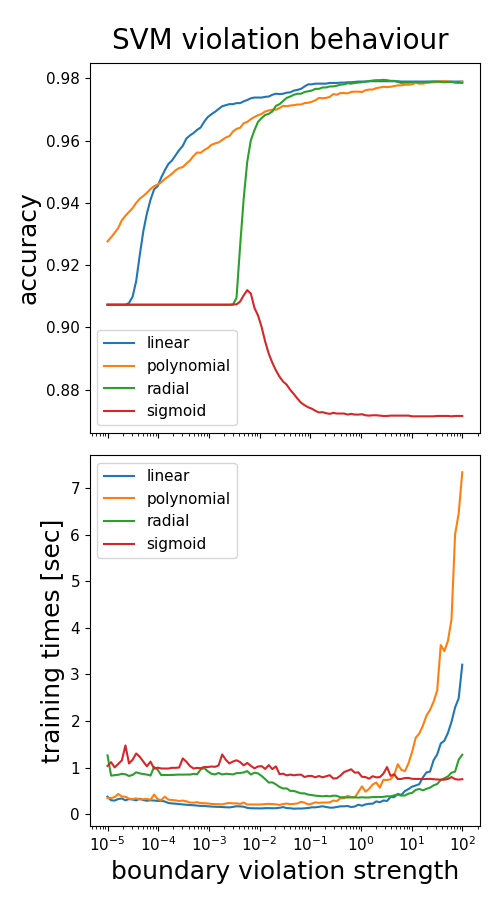
\includegraphics[scale=0.41]{../results/SVM/img/violation3.png}
\caption{A crude analysis of how the different SVM kernels behave with respect to different violation strengths.}\label{fig:SVM:violation}
\end{figure}
\begin{figure}[h!]
\centering
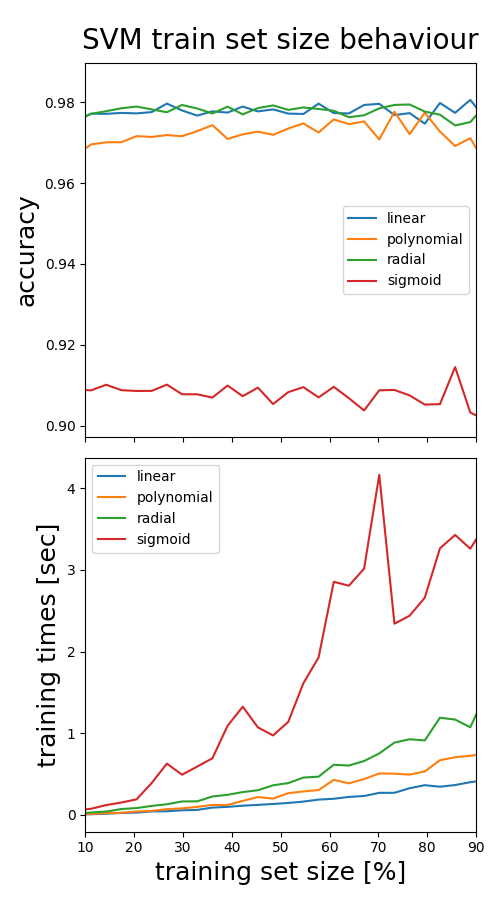
\includegraphics[scale=0.41]{../results/SVM/img/trainsetsize2.png}
\caption{A crude analysis of how the different SVM kernels behave with respect to different training set sizes.}\label{fig:SVM:training_set_size}
\end{figure}
\newpage

\subsubsection{Kernel hyperparameters}
The results for the SVM kernel hyperparameter analyses are shown in figures \ref{fig:SVM:kernel_polynomial}, \ref{fig:SVM:kernel_radial} and \ref{fig:SVM:kernel_sigmoid}. The three kernels exhibit quite different behaviour with respect to their respective hyperparameters. 

The accuracy of the polynomial kernels generally increase with increasing polynomial shift until about \(r\approx10^1\), where most of the kernels exhibit some form of maximum or peak accuracy (although the \(2^\text{nd}\) degree kernel could still be on the rise, the details are somewhat unclear). When it comes to training times, increasing the degree of the polynomial has more or less a blatant negative effect. Out of the different polynomial kernels, the \(3^\text{rd}\) degree polynomial stands out as both very effective, yet highly accurate (which is lucky considering the polynomial kernel used in the two previous analyses were both of degree 3).

Out of the different SVM kernels, the radial Gaussian SVM is sepecial in that it features a \emph{very clear} optimal hyperparameter, in fact a scaling factor of just about \(\gamma=10^{-1}\). This scaling both maximizes accuracy and minimizes training time, with little to no cost.

On the other hand, the Sigmoid SVM accuracy is more or less completely invariant of the argument shift \(r\). However, the training times make a hard drop around \(r\approx10^1\). Hence, a large \(r\), say \(r=10^3\), is clearly benefitial.

\begin{figure}[b!]
\centering
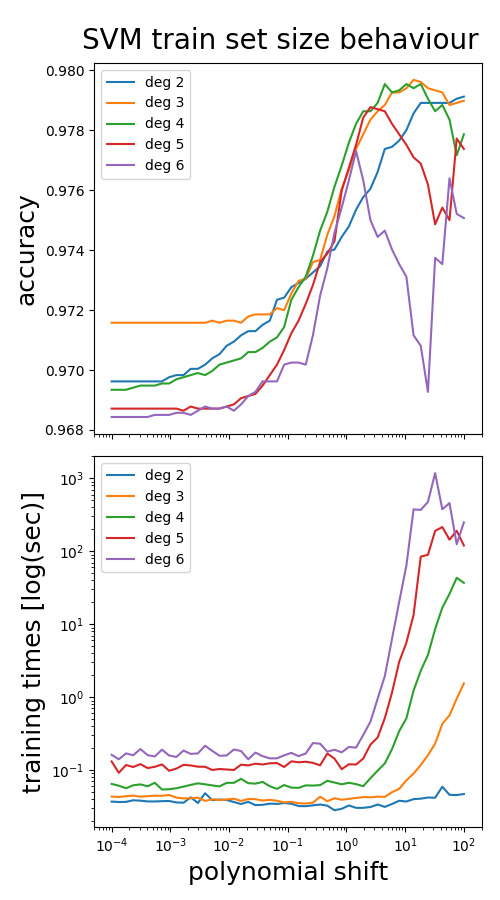
\includegraphics[scale=0.44]{../results/SVM/img/polynomial2.png}
\caption{Hyperparameter analysis of the polynomial SVM kernel.}\label{fig:SVM:kernel_polynomial}
\end{figure}

\begin{figure}[h!]
\centering
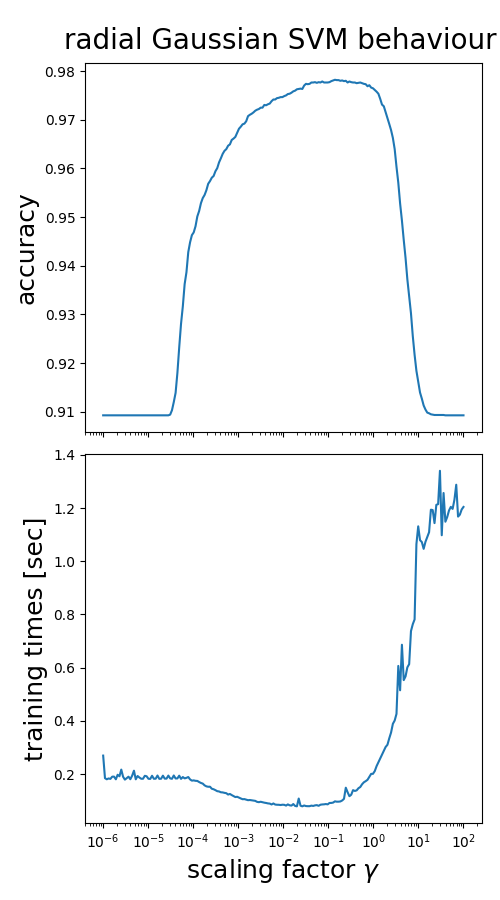
\includegraphics[scale=0.44]{../results/SVM/img/radial1.png}
\caption{Hyperparameter analysis of the radial Gaussian SVM kernel.}\label{fig:SVM:kernel_radial}
\end{figure}

\begin{figure}[b!]
\centering
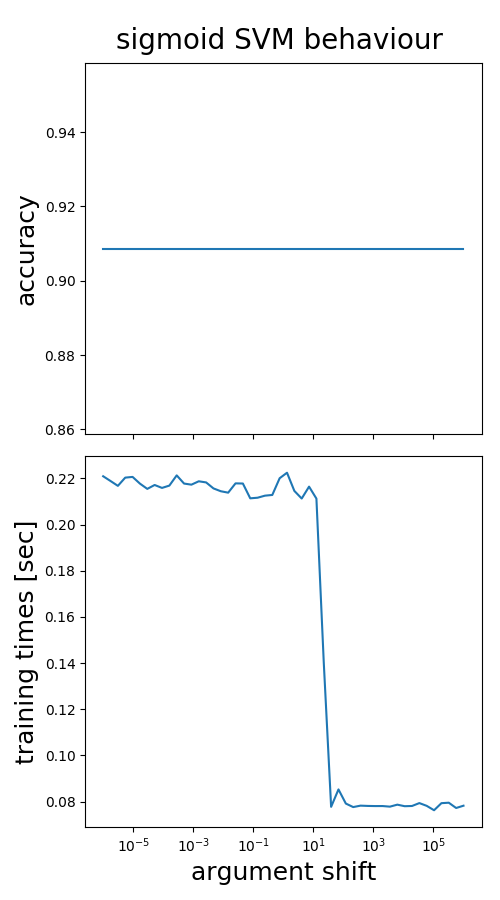
\includegraphics[scale=0.44]{../results/SVM/img/sigmoid1.png}
\caption{Hyperparameter analysis of the sigmoid SVM kernel.}\label{fig:SVM:kernel_sigmoid}
\end{figure}
\clearpage

\section{Discussion}
The goal of this project is to examine whether neural networks and support vector machines could be introduced as a standard tool for examining large data sets in radio astronomy. In particular whether these methods can be used to extract pulsar candidates from radio signals using their integrated pulse profiles and DM-SNR curves. Bathes et. al.'s 2012 attempt yielded an MLP network that was able to \emph{``blindly''} detect 85\% of pulsar candidates. However, as the results of this project has shown, the methods discussed in this project have the potential to improve his accuracy to as high as 98\%.

When it comes to the neural networks, it was clear that less complex networks, i.e. networks with less than about 10 layers, generally performed just as well as the more complex networks. In addition, the smaller network structures required much less training in general. An intersting case was the logistic networks, which required either a single layer or 2 layers in order to perform optimally. Overall, all network activation functions yielded good results, if parametrised correctly.

Nonetheless, based on the variety of acceptable hyperparameters that optimized the networks, the sigmoid networks definitely stood out as the most easy to work with. Especially considering that their training times were not particularly larger than the other two network activations. The sigmoid networks also performed very well for almost all choices of learning parameters, something that the logistic and rectifier networks did not. In fact, the sigmoid network is very stable for most combinations of hyperparameters; performing not only adequately, but exceptionally well.

Provided reasonable violation strengths, the support vector machines proved reasonble adversaries for the nerual networks; also scoring as high as 98\%. This was not true for every kernel however, the sigmoid kernel was not even able to score 92\%, which for comparison was the worst score for the other kernels.

Apart from the linear kernel, which was by far both the fastest and most accurate SVM, both the radial Gaussian and the \(3^\text{rd}\) degree polynomial kernels achieved an accuracy score of 98\% using less than a second to train. The polynomial SVM is trained slightly faster than the radial Gaussian SVM, but this is only measureble for \emph{very} large training sets. Judging by the separability of the pulsar data set (see histograms in appendix \ref{app:predictor_histograms}), the data set is most likely linear in its boundary. However, the radial Gaussian and polynomial SVMs are much more flexible than the linear SVM. In case a less linearly separable data set is used, the linear SVM is discouraged.

In general, the SVMs have exhibited slightly longer training times than the neural networks. Thus, neural networks could be adventageous in case training efficiency is important. However, the neural networks tend to have many more hyperparamaters, making the hyperparameter analysis that follows much more demanding than for an SVM. Take for instance the radial Gaussian SVM whose only hyperparameters are the violation strength and the scaling factor, and for comparison, a sigmoid neural network, which requires both a network structure analysis and a learning rate analysis. Assuming a hyperparameter analysis is required, training the SVM is likely much faster than training the neural network. On the other hand, the neural network is very robust, meaning a much smaller size of hyperparameter ranges may be used.

%It is important to address the fact that the data set considered in this project had already been analysed. In fact, the original raw data set consisting of the radio signals' IPPs and the DM-SNR curves were analysed and converted to statistical measures. This is not a negative however as this sort of practice is a common approach for many data mining analyses of time-varying signals.

\section{Conclusion}
In conclusion, the results of this project have shown that both neural networks and SVMs can be efficiently trained to correctly label some 98\% pulsars and non-pulsars in a data set consisting of statistical measures radio signals' IPPs and DM-SNR curves. Neither neural networks not SVMs stand out as the better alternative.

Designing a neural network for this purpose, it has been shown that using sigmoid activation, a small number of layers (\(\approx2\)) and few nodes \(\approx20\pm5\)) is likely to optimize the network for almost any choice of the initial learning rate and learning momentum strength. 

Designing an SVM for this purpose, it has been shown that the best results were produced using a linear kernel. However, this finding is most likely due to the linearly separability of the specific pulsar data set analysed in this project. Hence, if more flexibile SVMs are needed, it has been shown that similarly accurate results have been produced using a radial Gaussian with a violation of \(C=1\) and scaling factor \(\gamma=0.1\), and using a \(3^\text{rd}\) degree polynomial kernel with a violation of \(C=0.1\) and polynomial shift of \(r=10\).


%\bibliographystyle{plain}
\bibliographystyle{unsrtnat}
\bibliography{references.bib}


~
\appendix

\onecolumngrid
\section{Distributions of the Pulsar Data Set Predictors}\label{app:predictor_histograms}
\vspace{1.0cm}
\begin{figure}[h!]
\centering
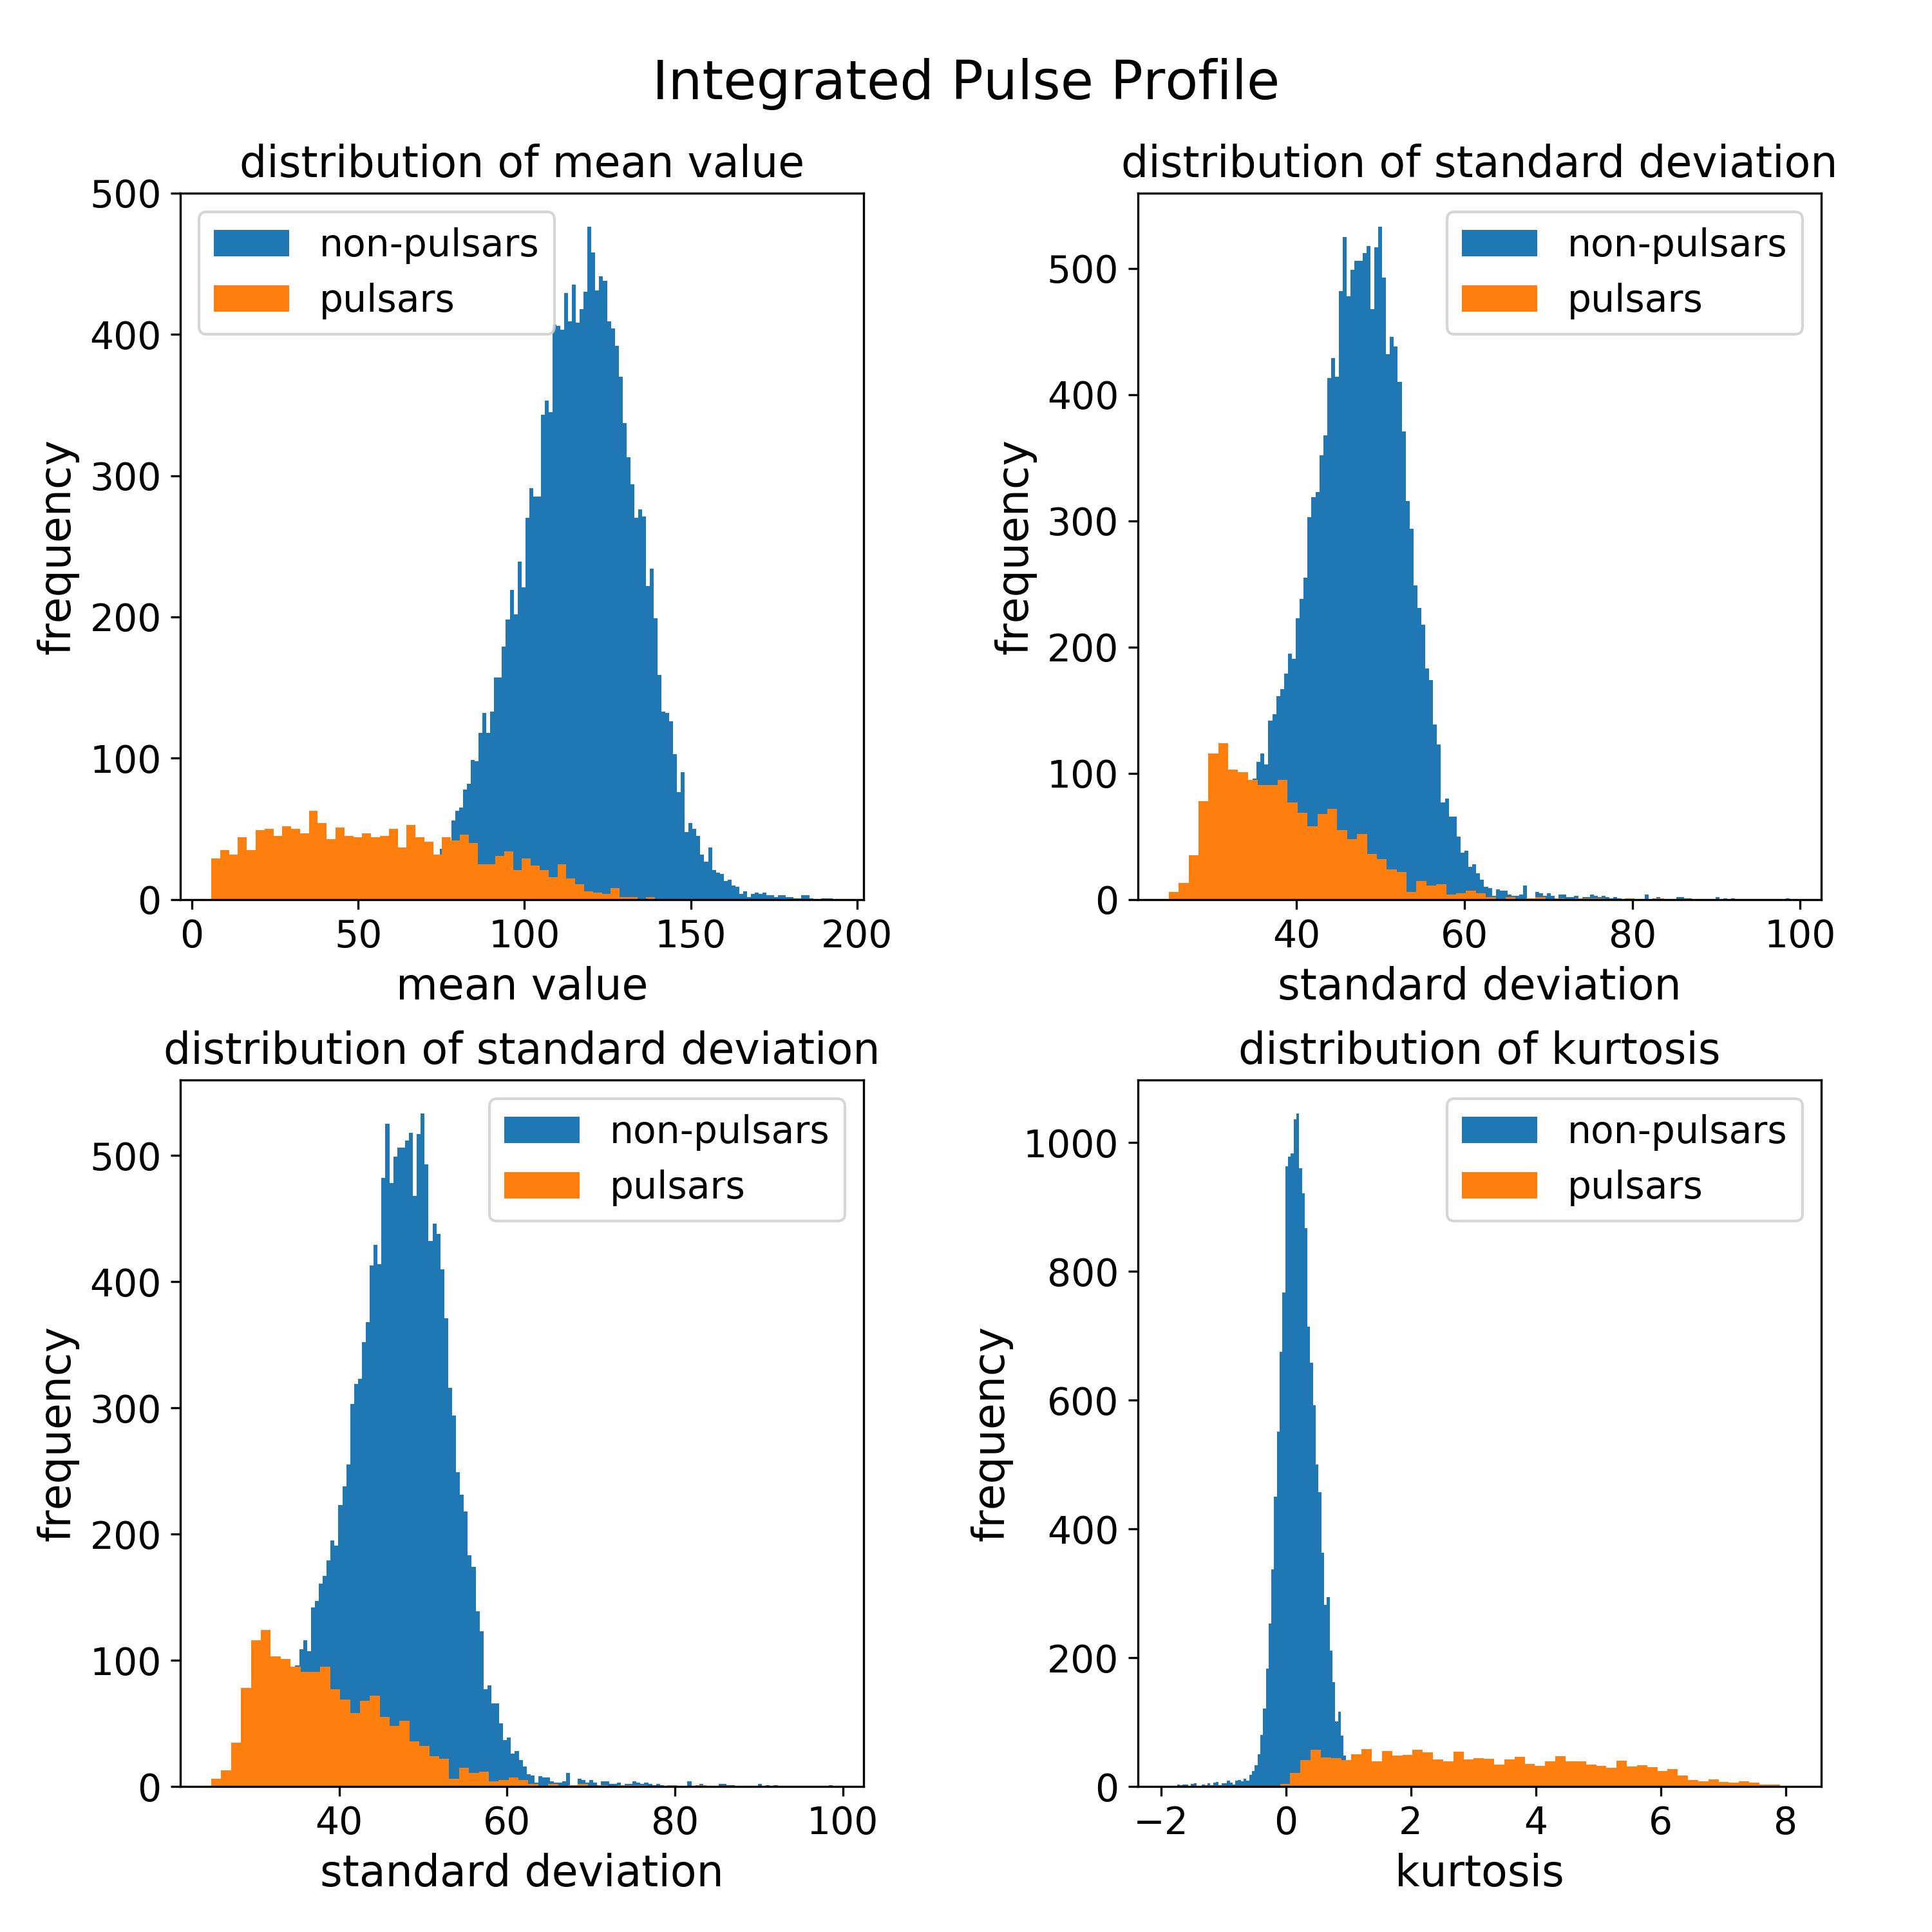
\includegraphics[scale=0.7]{../results/inspection_figures/IPP.png}
\caption{Histograms of the IPP predictors in the pulsar data set. The pulsars have been separeated from the non-pulsars in order to highlight the measurable difference between the two classes.}
\label{fig:IPP_predictors}
\end{figure}
\newpage
~

\vspace{2cm}
\begin{figure}[h!]
\centering
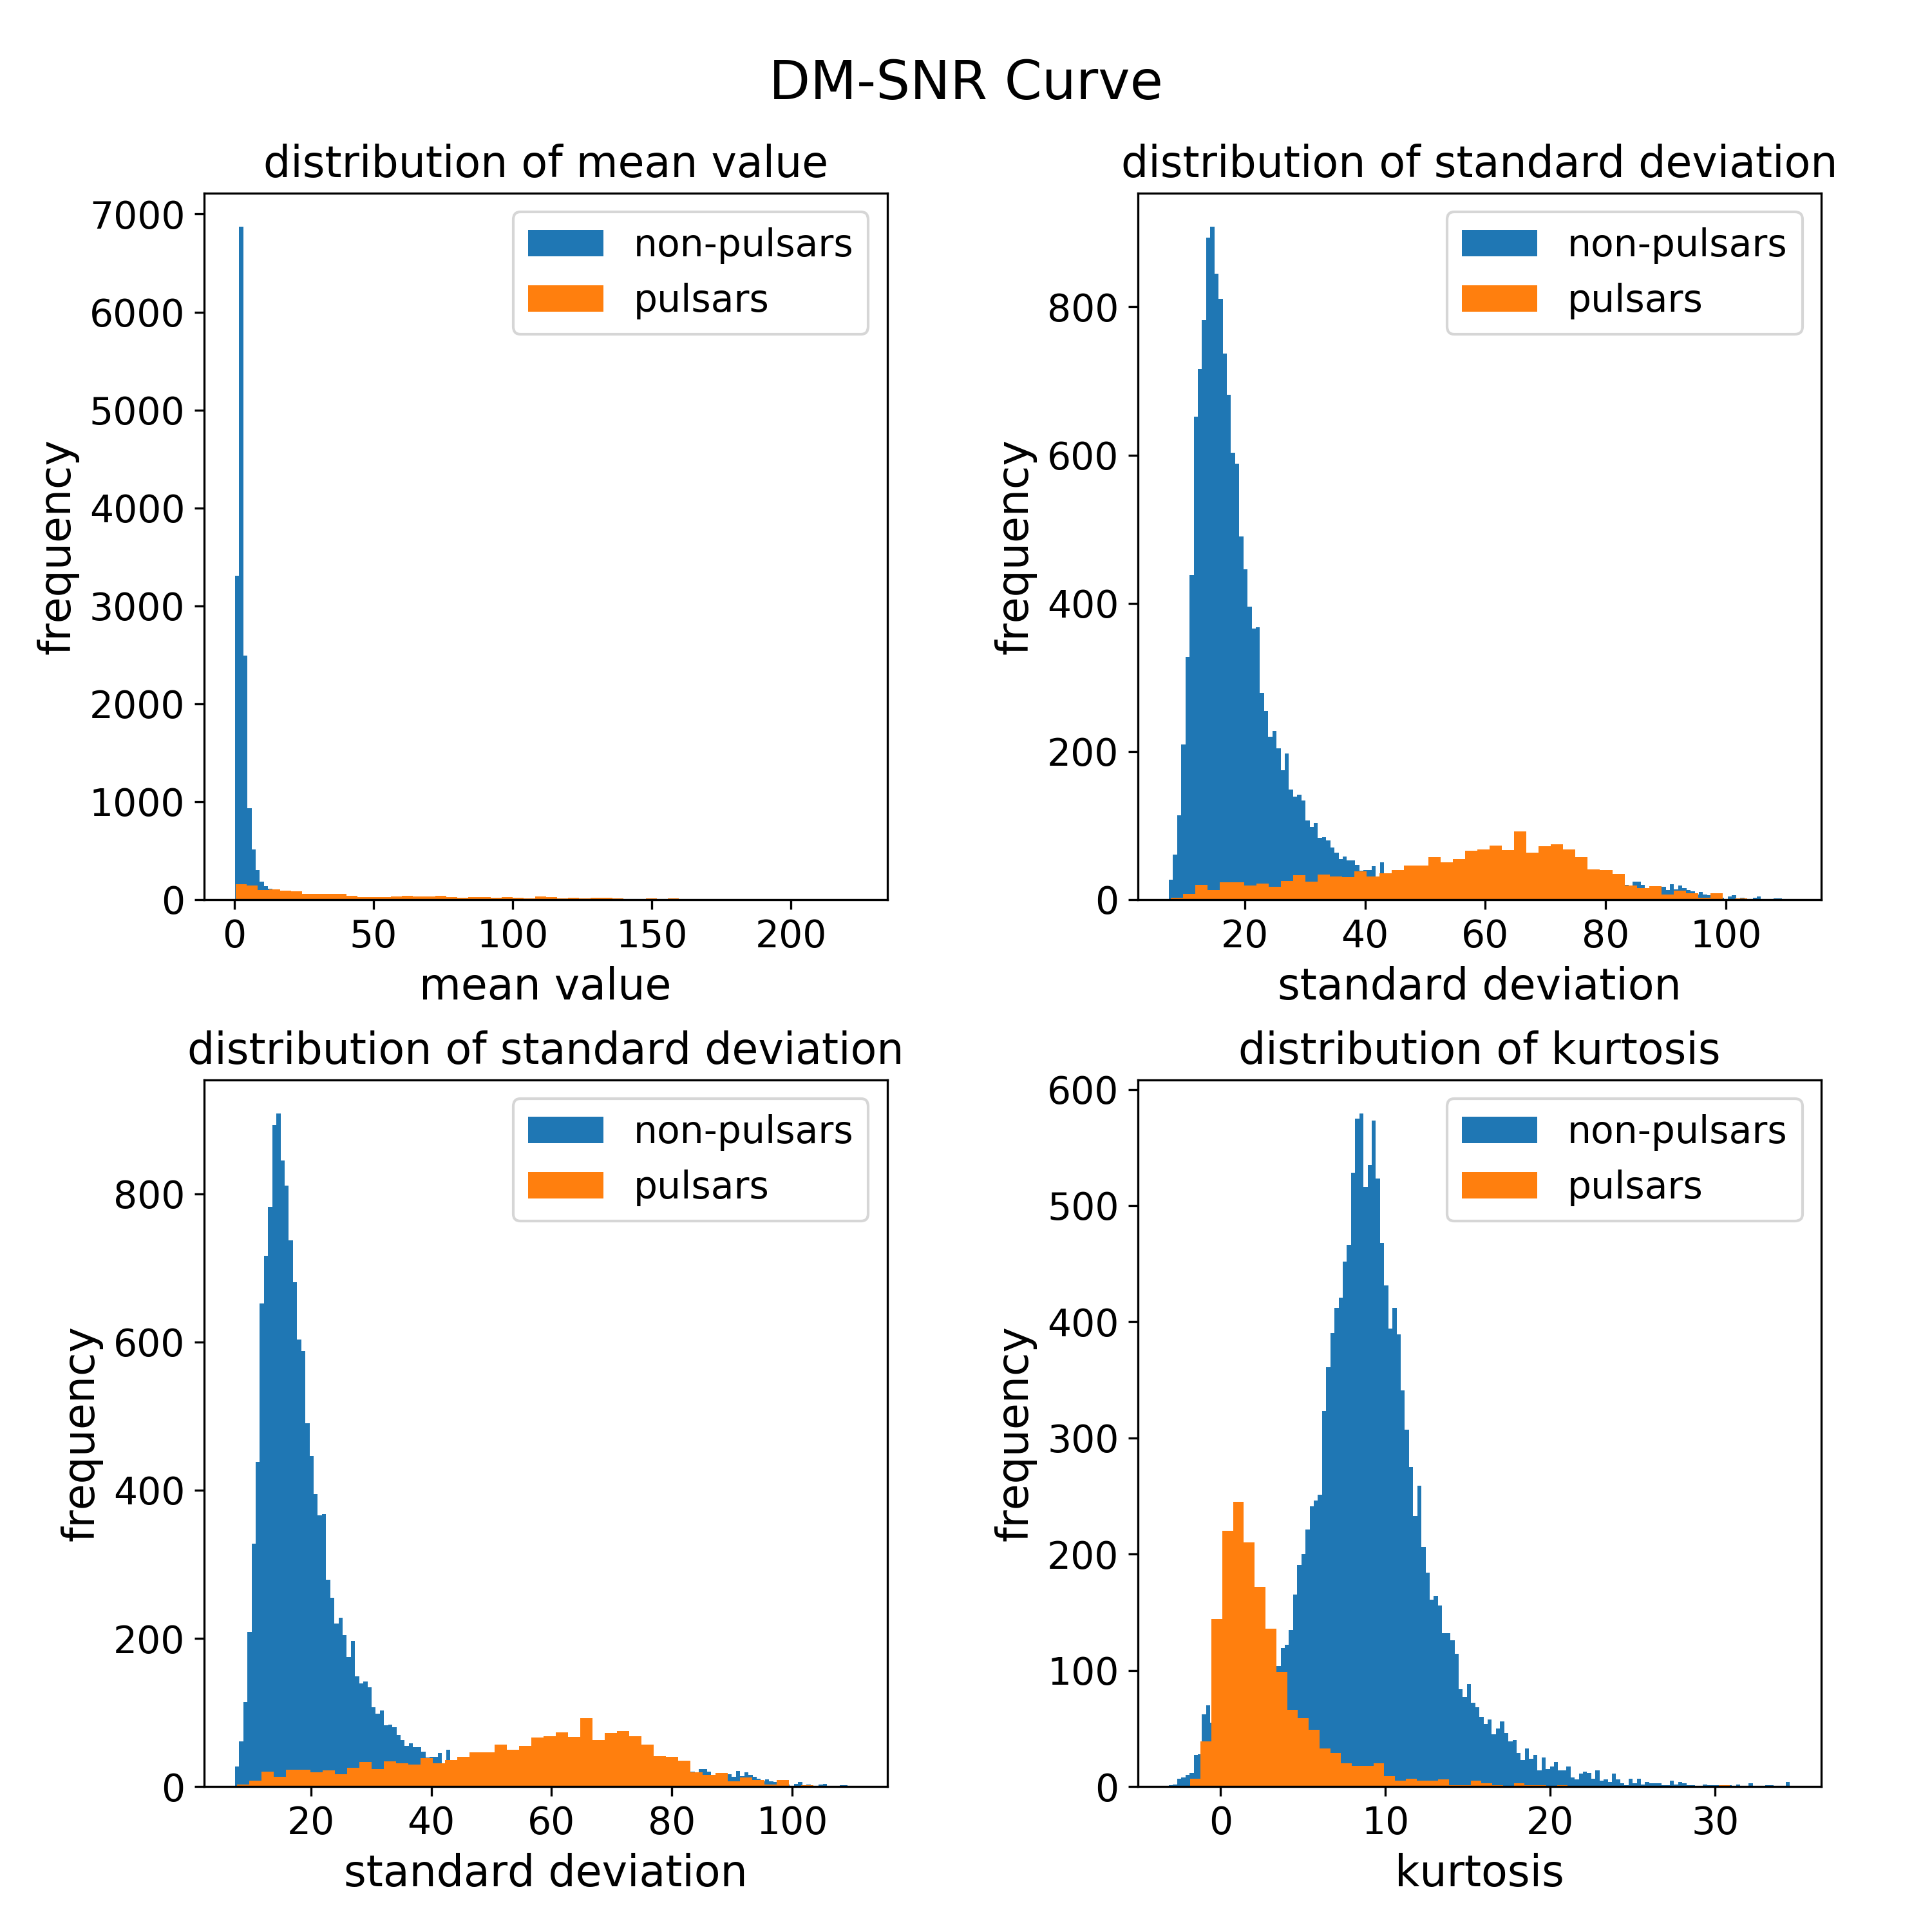
\includegraphics[scale=0.7]{../results/inspection_figures/SNR.png}
\caption{Histograms of the DM-SNR curve predictors in the pulsar data set. The pulsars have been separeated from the non-pulsars in order to highlight the measurable difference between the two classes.}
\label{fig:IPP_predictors}
\end{figure}








\end{document}